\documentclass[12pt]{article}
% Load necessary packages
\usepackage{abstract, adjustbox, amsmath, amssymb, amsthm, arydshln, bbm, booktabs, threeparttable, caption, color, 	colortbl, comment, csquotes, enumitem,  epstopdf, eurosym, float, framed, graphicx, graphics, 	hyperref, longtable, makebox, multirow, multicol, pdflscape, pdfpages, rotfloat, rotating, setspace, 	siunitx, soul, subcaption, tabularx, tablefootnote, tcolorbox, tikz, titling, verbatim, xcolor, xparse, xr, xurl, makecell}

\usetikzlibrary{calc, fit, patterns}
\usepackage[super]{nth}

% Geometry setup
\usepackage[left=1.25in, right=1.25in, top=1.25in, bottom=1.25in, head=0pt]{geometry}

% Bibliography style
\bibliographystyle{chicago}
\usepackage[longnamesfirst, authoryear]{natbib}

% Hyperref setup
\hypersetup{colorlinks=true, allcolors=blue, pdfstartview={FitV}, pdfpagemode={UseNone}, pdfnewwindow=true}

% Caption setup
\captionsetup[figure]{format=plain, width=1\textwidth, labelfont=bf, name=Figure, labelsep=newline, justification=justified}
\captionsetup[table]{format=plain, labelfont=bf, labelsep=newline, justification=justified}
\captionsetup[subfigure]{format=plain, position=top, labelsep=colon, labelformat=simple, labelfont=normalfont, justification=justified}

% Custom commands and environments
\newcommand\cites[1]{\citeauthor{#1}'s\ (\citeyear{#1})}
\newcommand{\ff}{\!f\!f}
\newcommand{\thinmidrule}{\midrule[0.15pt]}
\newtheorem{prop}{Proposition}
\def\sym#1{\ifmmode^{#1}\else\(^{#1}\)\fi}

\newenvironment{ltable}{\begin{landscape}\begin{table}}{\end{table}\end{landscape}}
\newenvironment{lfigure}{\begin{landscape}\begin{figure}}{\end{figure}\end{landscape}}

% Siunitx setup
\sisetup{
	%detect-mode,
	%tight-spacing           = true,
	%group-digits            = false,
	%input-signs             = ,
	%input-symbols           = ,
	input-open-uncertainty  = ,
	input-close-uncertainty = ,
	table-align-text-pre    = false,
	%round-mode              = figures,
	%round-precision         = 3,
	table-space-text-pre    = (,
	table-space-text-post   = ),
	round-mode=places, 
	round-precision=3
}

% Section and Subsection numbering
\renewcommand{\thesection}{\arabic{section}}  
\renewcommand{\thesubsection}{\thesection.\arabic{subsection}}
\renewcommand{\thetable}{\arabic{table}}
\renewcommand{\thesubfigure}{\Alph{subfigure}}


\title{Hedge Funds Strategies}
\author{Davide Tomio}
\date{June 2025}

\begin{document}

\maketitle

\section{Data}

I have gotten the following data
\begin{itemize}
    \item Bond prices, these are all bonds issued by DE IT FR ES + US
    \begin{itemize}
        \item I calculated yields, duration, and convexity for all.
        \item I exported the files.
        \item I calculated the noise measure. For this, I eliminated bonds where my estimated yield and the ECB yield was more than 5bp apart, and bonds that had a pricing error larger than 50bp
        \item I calculated noise measure and fitted prices under both Svensson and Nelson Siegel (NS seems to perform better)
    \end{itemize}
    \item Repo.
    \begin{itemize}
        \item Felix provided fund-by-bond-by-day positions, both buy and sell
    \end{itemize}
    \item Policy surprises form Altavilla et al (Measuring euro area monetary policy)
    \end{itemize}

\section{Analysis}
\begin{itemize}
    \item Do they make money around monetary policy announcements? 
    \begin{enumerate}
        \item Focus on Germany (other countries have credit risk stuff)
        \item To test level: Aggregate total duration for the HF business, is it higher right before positive (higher than expected IR) news? Important to somehow scale it. Is it negative before negative (lower than expected) IR? Does it revert after news? 
        \item To test slope: Aggregate convexity? (Chen et al in ``In Search of Habitat'' refer to slope duration. Not sure how to calculate it.      
    \end{enumerate}
    \item Do they make money by shorting bonds? 
    \begin{enumerate}
        \item Are returns lower for bonds with high shorting? The issue with this is what about bonds that are flat and have experienced run-up, they should have high shorting before the price goes down. So maybe look forward? 
        \item Alternative average returns before, after, during a spell of more than 1\% shorting.
    \end{enumerate}
    \item Do they play term-structure arbitrage? 
    \begin{enumerate}
        \item Sort by shorting quintile, average their pricing error by date, following days.
    \end{enumerate}
    \item Do they ``convergence trade''? 
\end{itemize}t
\section{Next steps}
\begin{enumerate}[label=\arabic*.]
    \item Calculate duration for bonds and futures at the fund-day level
    \item Aggregate it to compare to OFR
    \item Show that they \textit{do} relative value trade
    \begin{enumerate}[label=\alph*.]
        \item In the aggregate
        \item Fund by fund (come up with a threshold for the delta or correlation) 
    \end{enumerate}
\end{enumerate}
    

\clearpage\newpage

\begin{figure}\captionsetup{width=1\textwidth}
	\caption{\bf CTD }
	\caption*{\footnotesize
     This figure 
}
		\includegraphics[width=1\linewidth]{Figures/exampleCTD.pdf}
\end{figure}



\begin{figure}\captionsetup{width=1\textwidth}
	\caption{\bf Retail Option Traes}
		\caption*{\footnotesize This figvely.}\centering
	\begin{subfigure}{0.8\linewidth}
		\caption{\(Yield - CurveYield_{it}\)	}\centering
		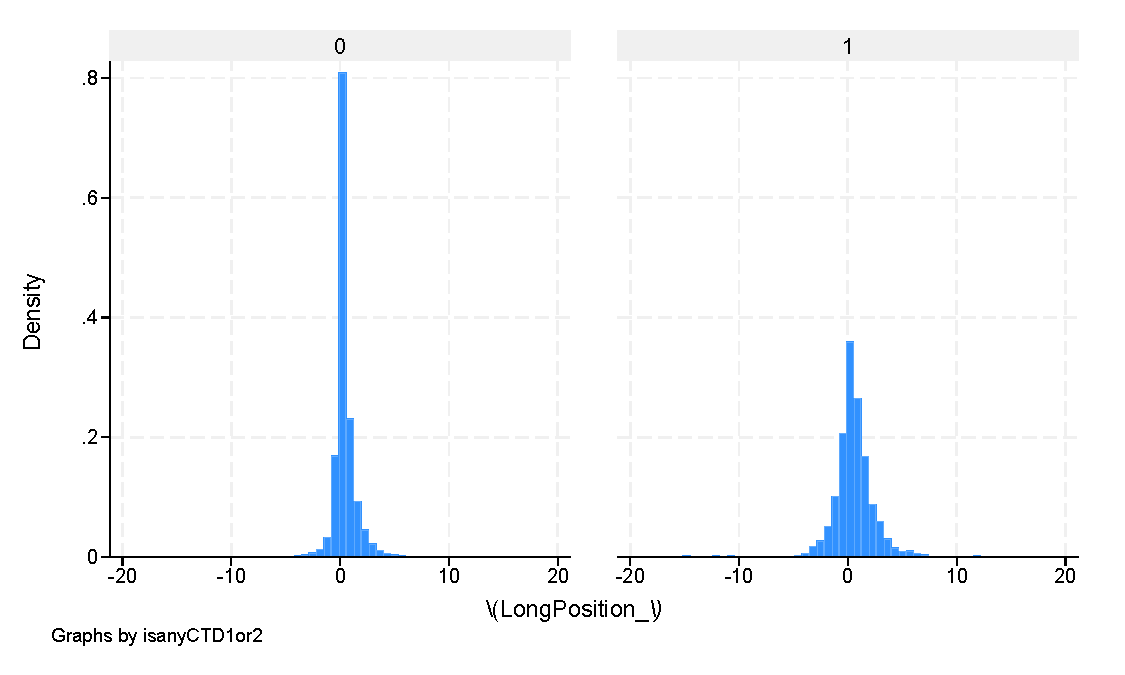
\includegraphics[width=1\linewidth]{Figures/distdyield.pdf}
	\end{subfigure}\\
		\begin{subfigure}{0.8\linewidth}
		\caption{Long}\centering
		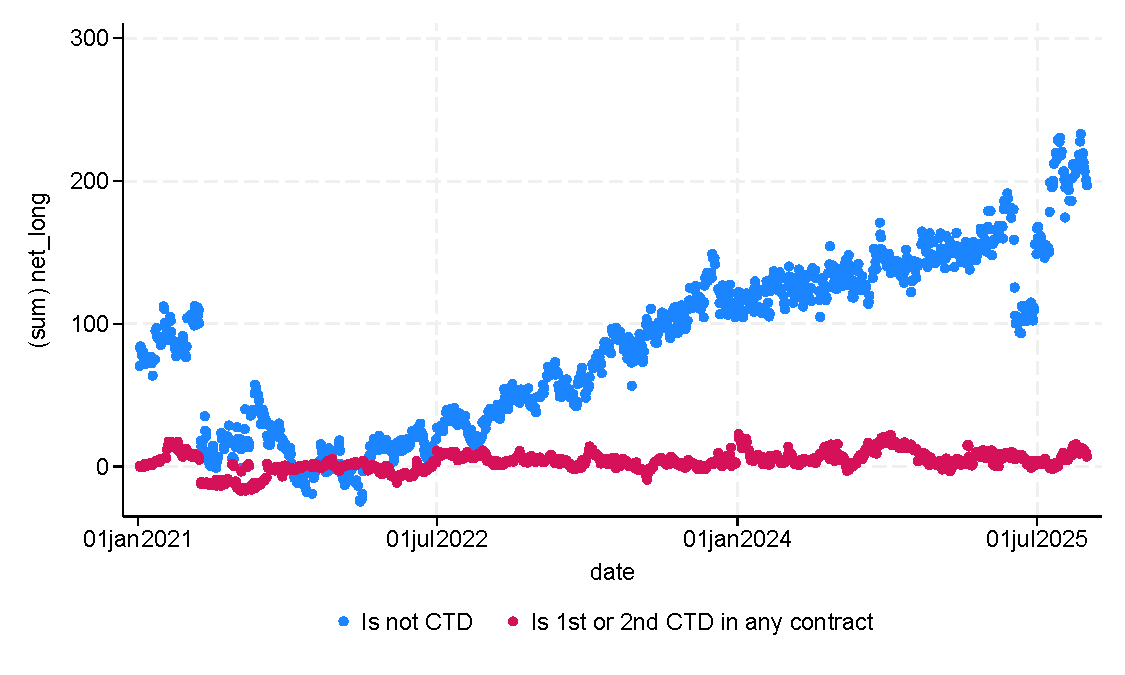
\includegraphics[width=1\linewidth]{Figures/distlong.pdf}
	\end{subfigure}
\end{figure}

\begin{figure}\captionsetup{width=1\textwidth}
	\caption{\bf Retail Option Traes}
		\caption*{\footnotesize This figvely.}\centering
	\begin{subfigure}{0.8\linewidth}
		\caption{\(Yield - CurveYield_{it}\)	}\centering
		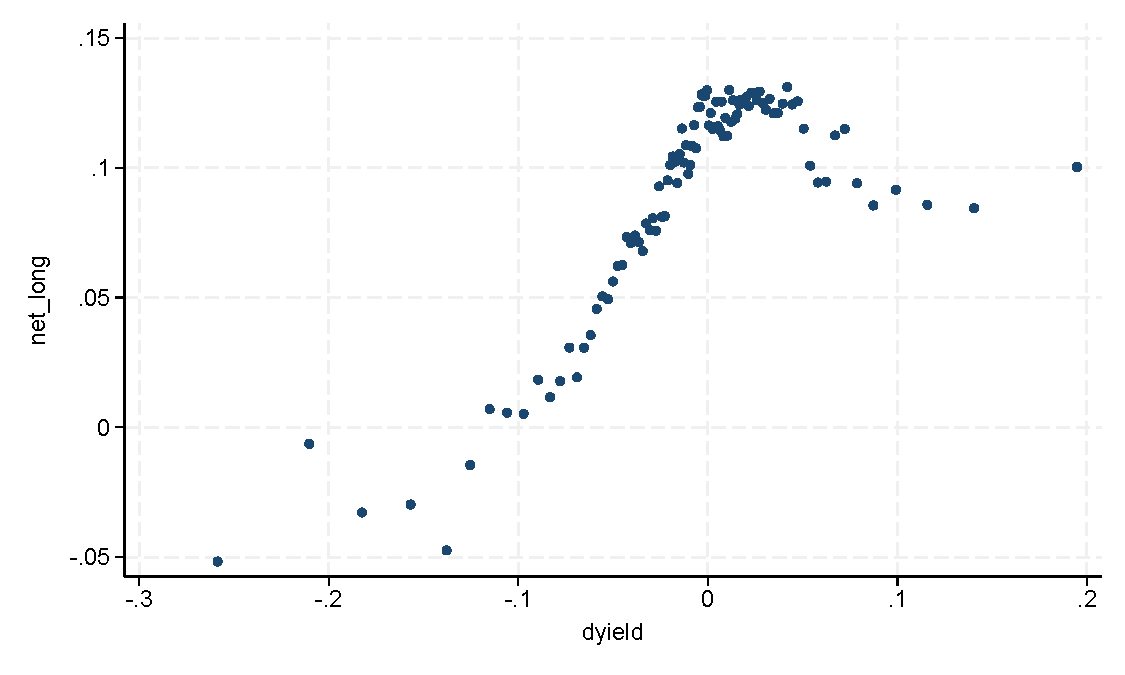
\includegraphics[width=1\linewidth]{Figures/dyieldnet_long1.pdf}
	\end{subfigure}\\
		\begin{subfigure}{0.8\linewidth}
		\caption{Long}\centering
		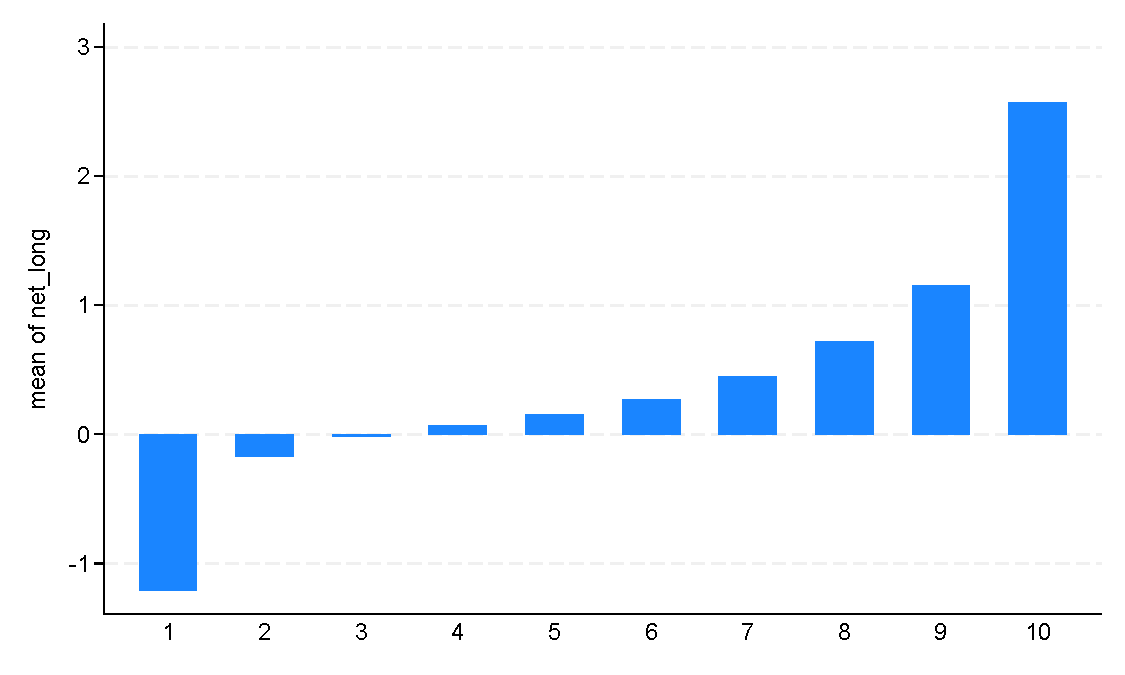
\includegraphics[width=1\linewidth]{Figures/dyieldnet_long2.pdf}
	\end{subfigure}
\end{figure}

\begin{figure}\captionsetup{width=1\textwidth}
	\caption{\bf Retail Option Traes}
		\caption*{\footnotesize This figvely.}\centering
	\begin{subfigure}{0.8\linewidth}
		\caption{US}\centering
		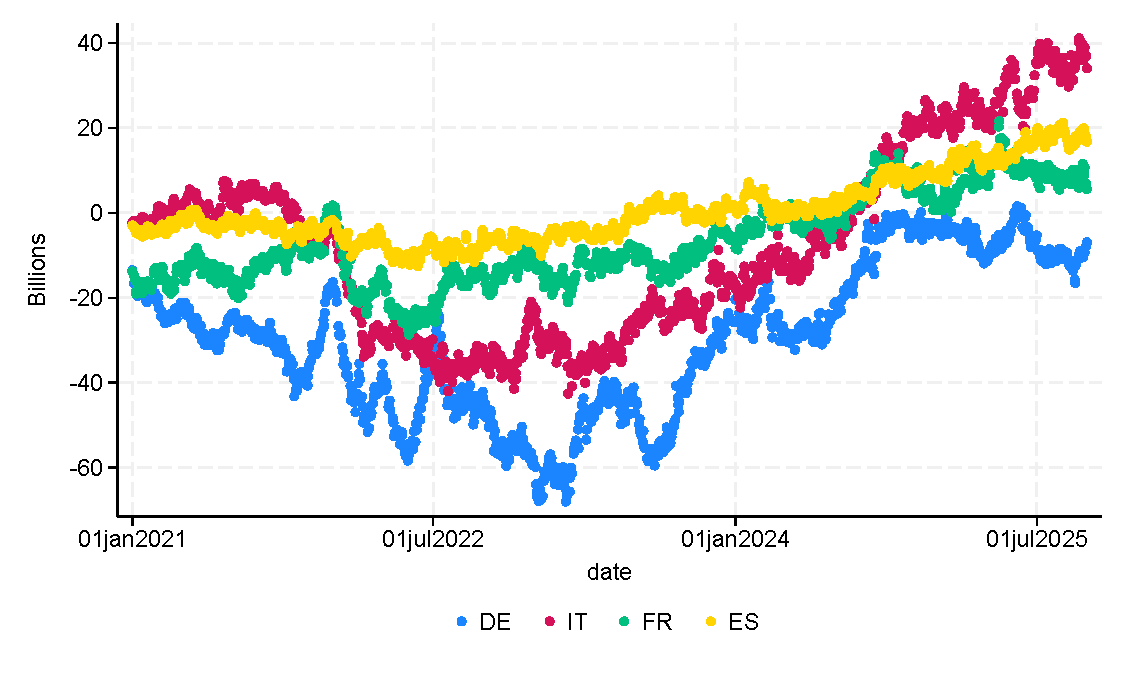
\includegraphics[width=1\linewidth]{Figures/net_long.pdf}
	\end{subfigure}\\
		\begin{subfigure}{0.8\linewidth}
		\caption{EU}\centering
		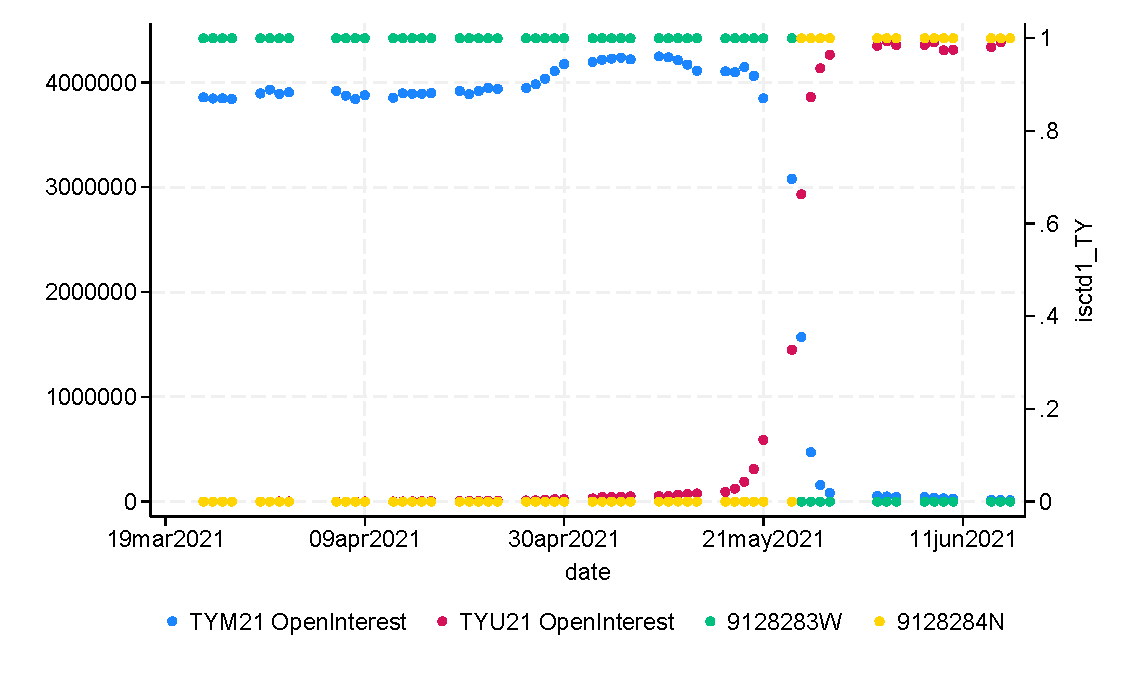
\includegraphics[width=1\linewidth]{Figures/eu_pos.pdf}
	\end{subfigure}
\end{figure}


\begin{figure}\captionsetup{width=1\textwidth}
	\caption{\bf Retail Option Traes}
		\caption*{\footnotesize This figvely.}\centering
		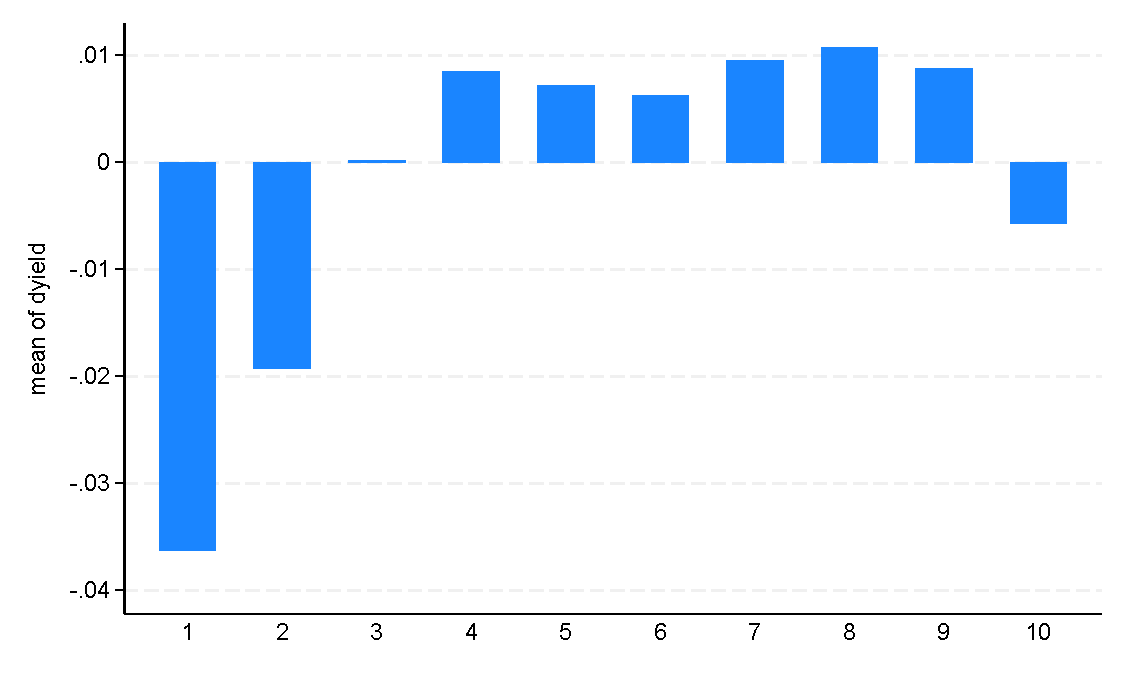
\includegraphics[width=1\linewidth]{Figures/net_longbyctd.pdf}
\end{figure}

\begin{figure}\captionsetup{width=1\textwidth}
	\caption{\bf Retail Option Traes}
		\caption*{\footnotesize This figvely.}\centering
	\begin{subfigure}{0.8\linewidth}
		\caption{Duration}\centering
		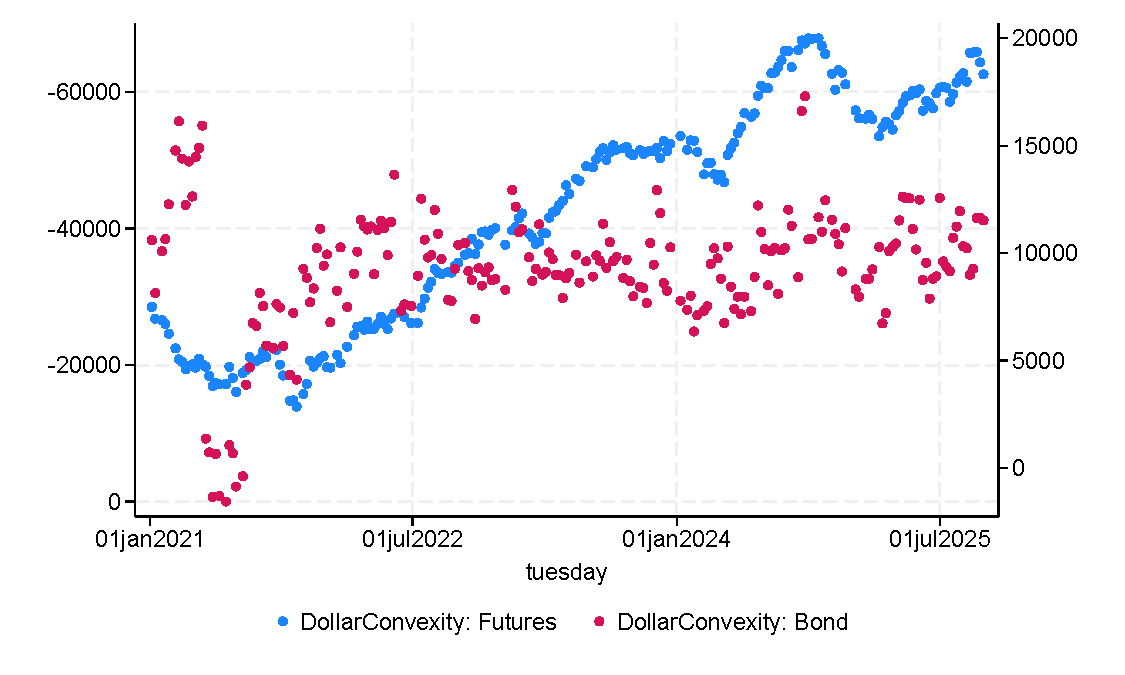
\includegraphics[width=1\linewidth]{Figures/dur1.pdf}
	\end{subfigure}\\
		\begin{subfigure}{0.8\linewidth}
		\caption{Convexity}\centering
		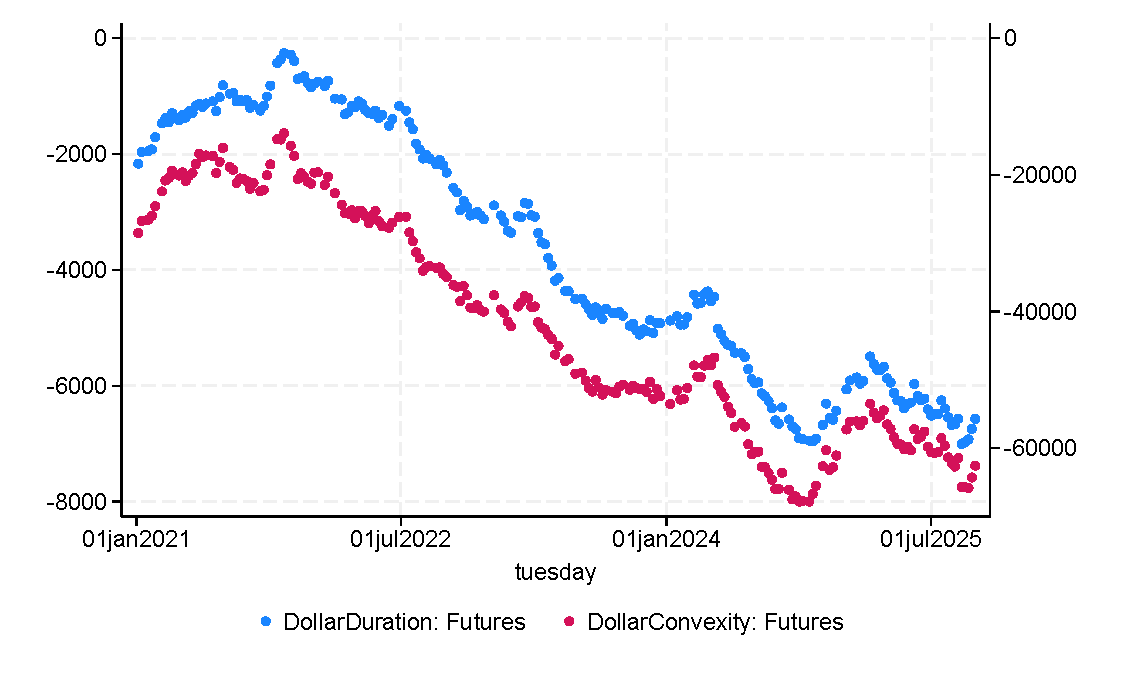
\includegraphics[width=1\linewidth]{Figures/con1.pdf}
	\end{subfigure}
\end{figure}

\begin{figure}\captionsetup{width=1\textwidth}
	\caption{\bf Retail Option Traes}
		\caption*{\footnotesize This figvely.}\centering
	\begin{subfigure}{0.8\linewidth}
		\caption{Duration}\centering
		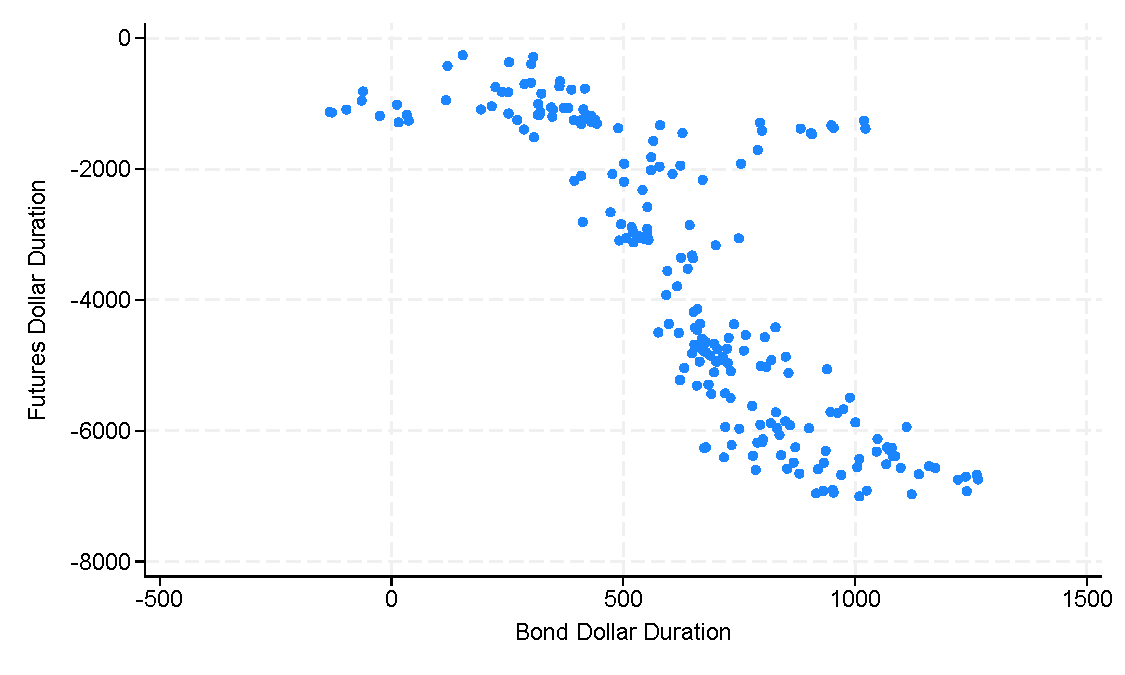
\includegraphics[width=1\linewidth]{Figures/bon1.pdf}
	\end{subfigure}\\
		\begin{subfigure}{0.8\linewidth}
		\caption{Convexity}\centering
		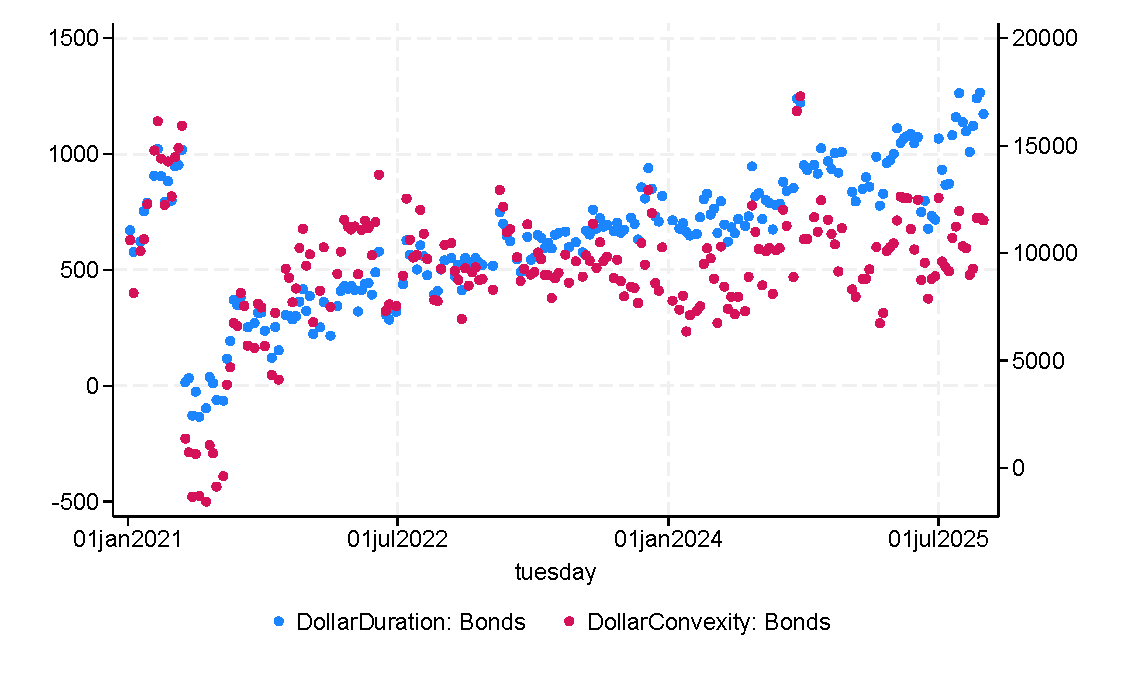
\includegraphics[width=1\linewidth]{Figures/fut1.pdf}
	\end{subfigure}
\end{figure}

\begin{figure}\captionsetup{width=1\textwidth}
	\caption{\bf Retail Option Traes}
		\caption*{\footnotesize This figvely.}\centering
	\begin{subfigure}{0.8\linewidth}
		\caption{Duration}\centering
		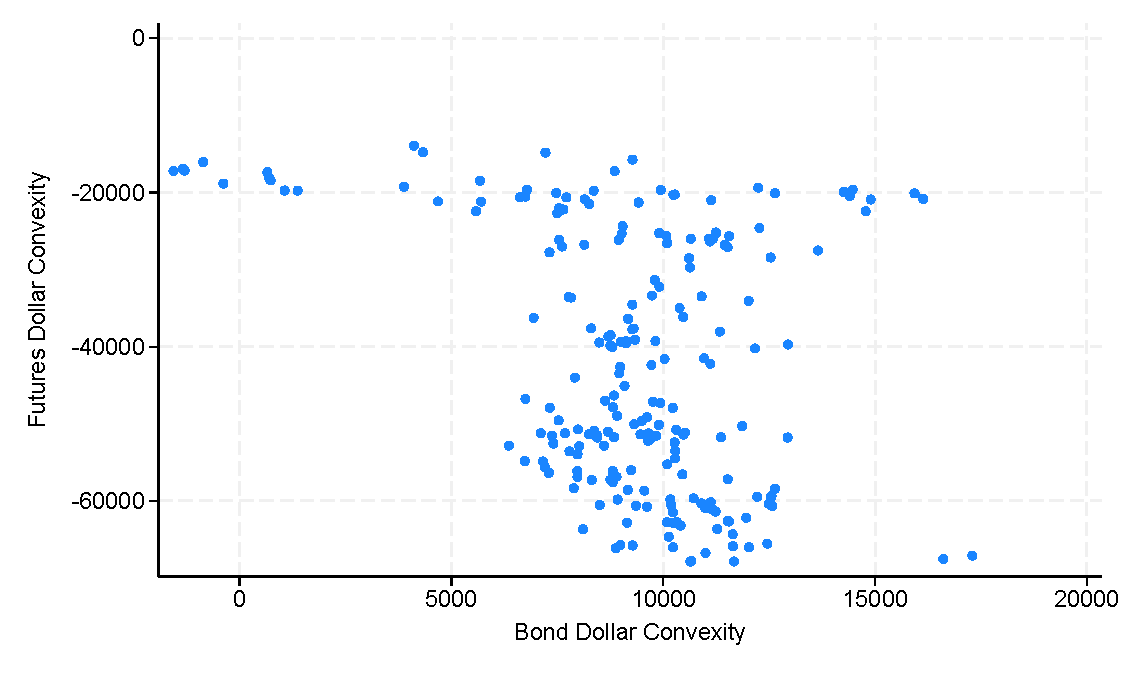
\includegraphics[width=1\linewidth]{Figures/dur2.pdf}
	\end{subfigure}\\
		\begin{subfigure}{0.8\linewidth}
		\caption{Convexity}\centering
		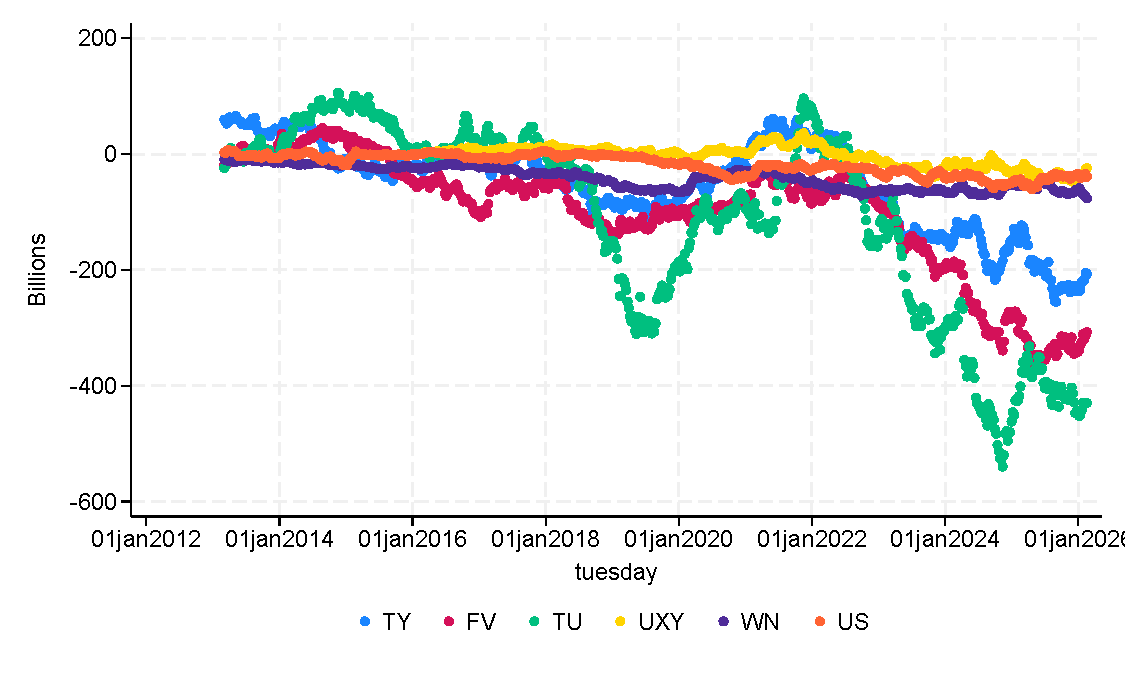
\includegraphics[width=1\linewidth]{Figures/con2.pdf}
	\end{subfigure}
\end{figure}

\begin{figure}\captionsetup{width=1\textwidth}
	\caption{\bf CTD }
	\caption*{\footnotesize
     This figure 
}
		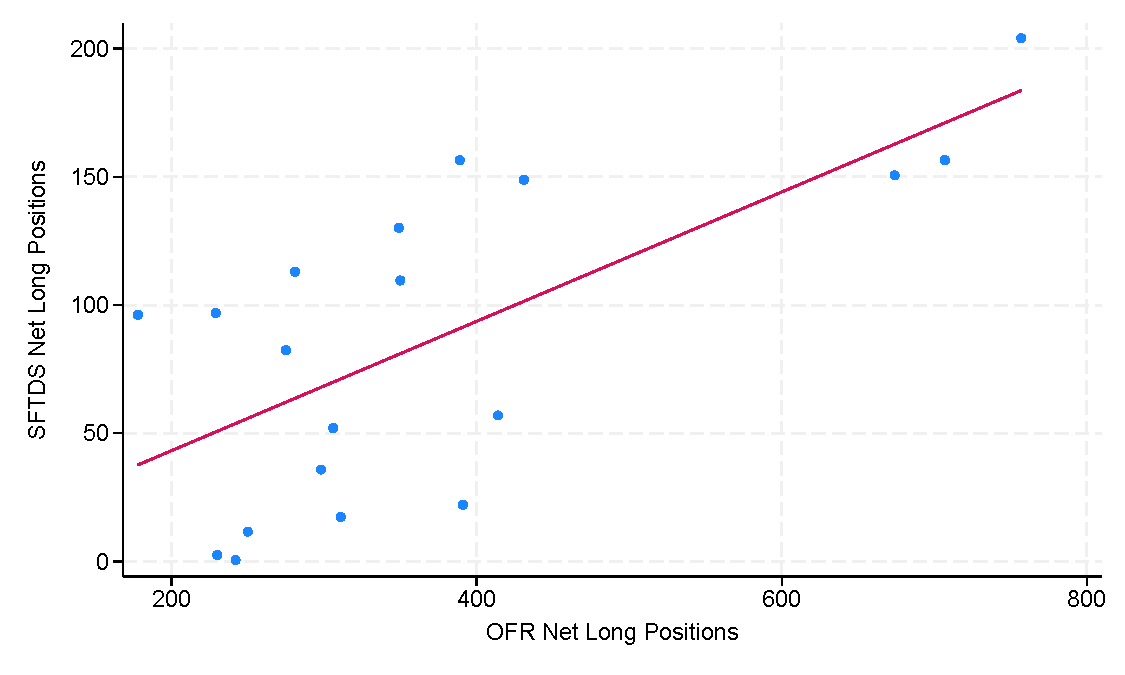
\includegraphics[width=1\linewidth]{Figures/futures_ts.pdf}
\end{figure}

\begin{figure}\captionsetup{width=1\textwidth}
	\caption{\bf CTD }
	\caption*{\footnotesize
     This figure 
}
		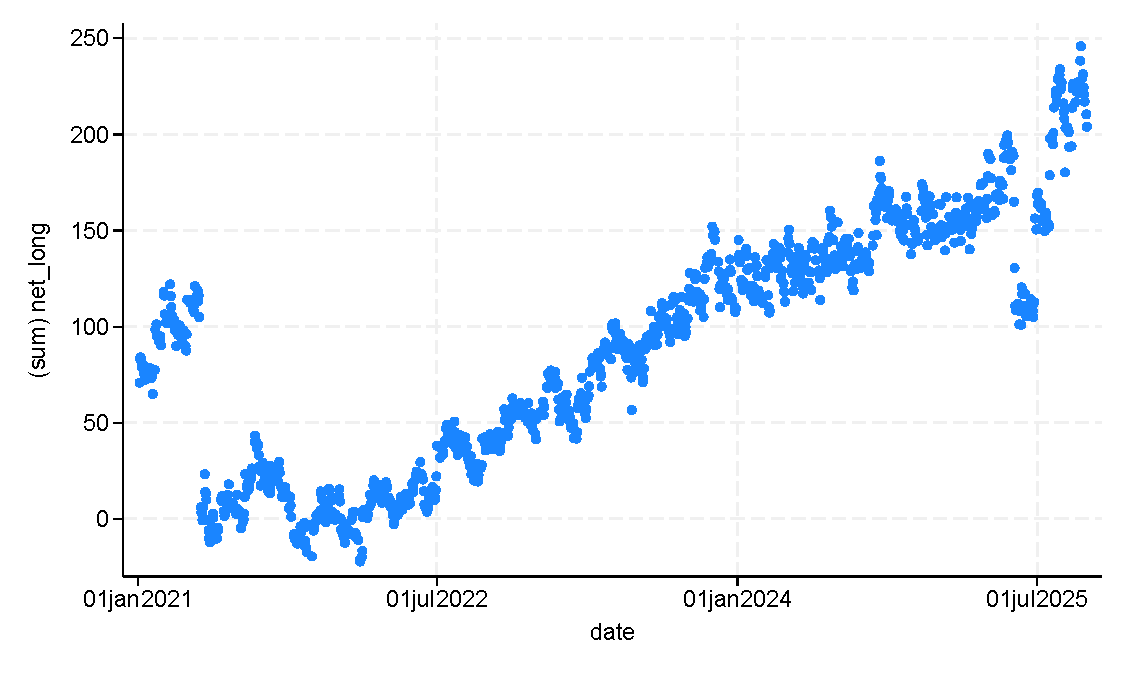
\includegraphics[width=1\linewidth]{Figures/ofrcomp.pdf}
\end{figure}

\clearpage\newpage
\begin{table}\centering\captionsetup{width=0.9\textwidth}\small
    \caption{\large \bf   R  res} 
    \caption*{\footnotesize	This  .}
     \resizebox{0.9\textwidth}{!}{{
\def\sym#1{\ifmmode^{#1}\else\(^{#1}\)\fi}
\begin{tabular}{l*{1}{S[table-format=4.3]S[table-format=4.3]S[table-format=4.3, table-space-text-post = {***}]}}
\toprule
                    &\multicolumn{1}{c}{\(FV CTD=0\)}&\multicolumn{1}{c}{\(FV CTD=1\)}&\multicolumn{1}{c}{Difference}   \\
\midrule
\(LongPosition_{it}\)&    .3965319&    .3800099&    -.016522   \\
\bottomrule
\end{tabular}
}
}
\end{table}	

\begin{table}\centering\captionsetup{width=0.9\textwidth}\small
    \caption{\large \bf   R  res} 
    \caption*{\footnotesize	This  .}
    {
\def\sym#1{\ifmmode^{#1}\else\(^{#1}\)\fi}
\begin{tabular}{l*{1}{S[table-format=4.3]S[table-format=4.3]S[table-format=4.3, table-space-text-post = {***}]}}
\toprule
                    &\multicolumn{1}{c}{\(TU CTD=0\)}&\multicolumn{1}{c}{\(TU CTD=1\)}&\multicolumn{1}{c}{Difference}   \\
\midrule
\(LongPosition_{it}\)&    .3962501&    .4601651&     .063915   \\
\bottomrule
\end{tabular}
}

    {
\def\sym#1{\ifmmode^{#1}\else\(^{#1}\)\fi}
\begin{tabular}{l*{1}{S[table-format=4.3]S[table-format=4.3]S[table-format=4.3, table-space-text-post = {***}]}}
\toprule
                    &\multicolumn{1}{c}{\(US CTD=0\)}&\multicolumn{1}{c}{\(US CTD=1\)}&\multicolumn{1}{c}{Difference}   \\
\midrule
\(LongPosition_{it}\)&    .3961285&    .4705815&     .074453** \\
\bottomrule
\end{tabular}
}

    {
\def\sym#1{\ifmmode^{#1}\else\(^{#1}\)\fi}
\begin{tabular}{l*{1}{S[table-format=4.3]S[table-format=4.3]S[table-format=4.3, table-space-text-post = {***}]}}
\toprule
                    &\multicolumn{1}{c}{\(UXY CTD=0\)}&\multicolumn{1}{c}{\(UXY CTD=1\)}&\multicolumn{1}{c}{Difference}   \\
\midrule
\(LongPosition_{it}\)&    .4004991&   -.5131415&   -.9136406***\\
\bottomrule
\end{tabular}
}

    {
\def\sym#1{\ifmmode^{#1}\else\(^{#1}\)\fi}
\begin{tabular}{l*{1}{S[table-format=4.3]S[table-format=4.3]S[table-format=4.3, table-space-text-post = {***}]}}
\toprule
                    &\multicolumn{1}{c}{\(WN CTD=0\)}&\multicolumn{1}{c}{\(WN CTD=1\)}&\multicolumn{1}{c}{Difference}   \\
\midrule
\(LongPosition_{it}\)&    .3944148&    .8557294&    .4613146***\\
\bottomrule
\end{tabular}
}

    \input{Tables/dUXY}
    \input{Tables/dWN}
\end{table}	
\newpage\clearpage


\section{Descriptives}

\begin{figure}\captionsetup{width=1\textwidth}
	\caption{\bf Distribution of counterparties per hedge fund}
	\caption*{\footnotesize
}
		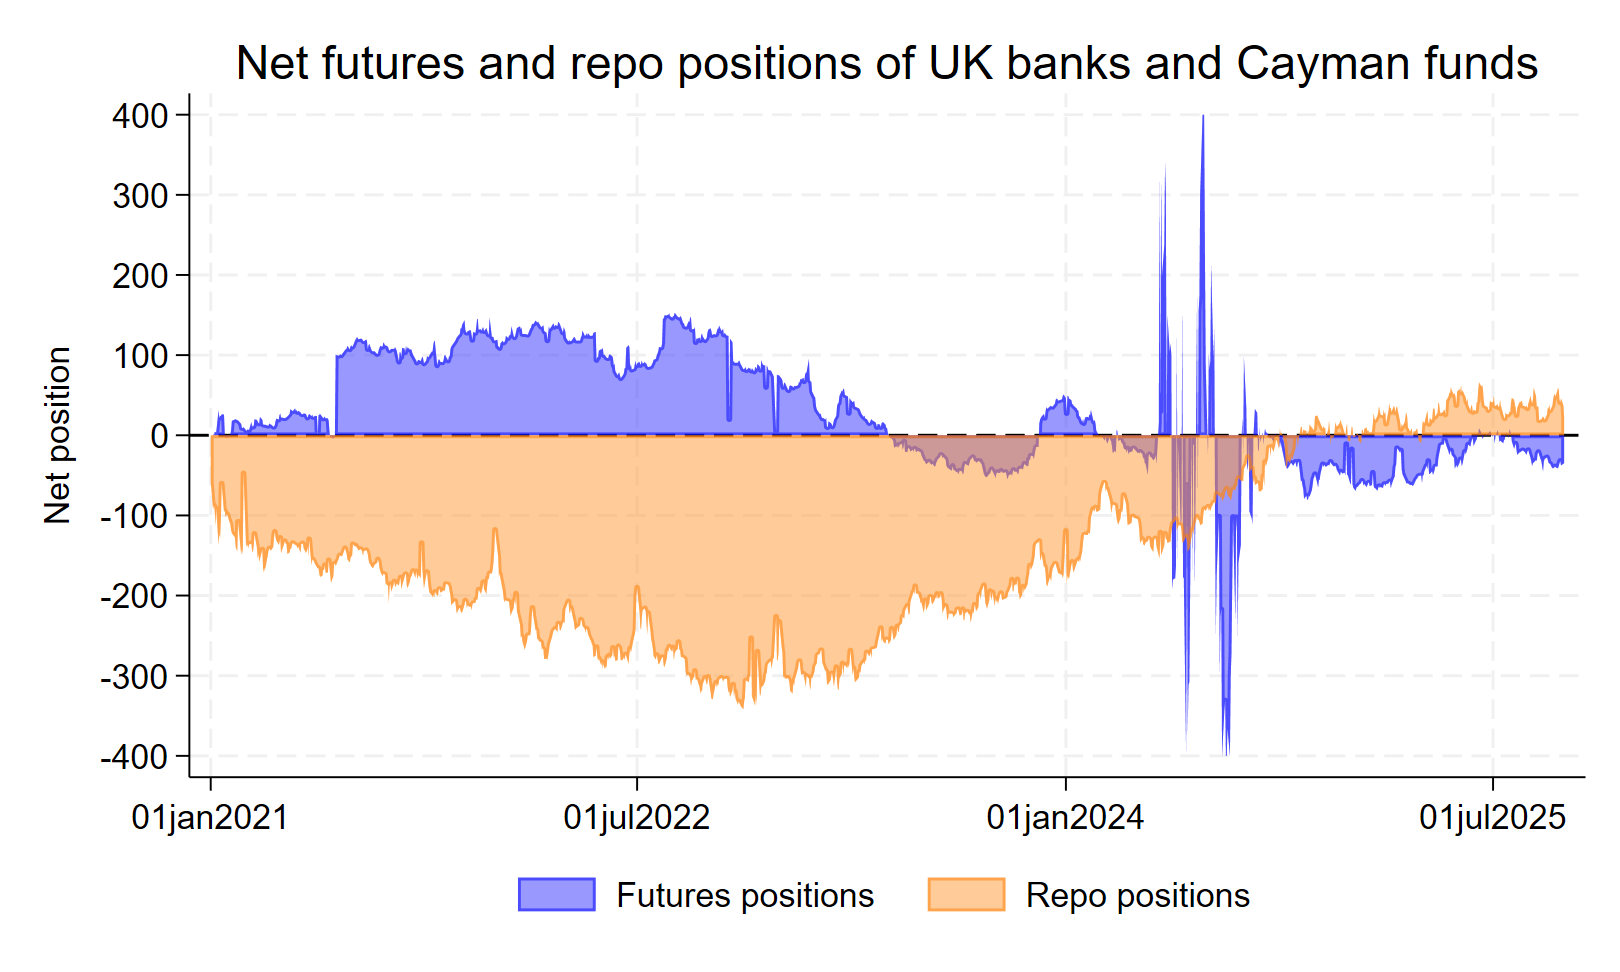
\includegraphics[width=1\linewidth]{Figures/distribution_HF_counterparties.png}
\end{figure}



\begin{table}[htbp]
\centering
\caption{Summary Statistics: Hedge Fund Activity in EUR and USD Repo Markets}
\label{tab:summary}
\small
\begin{tabular}{lcc}
\toprule
 & EUR & USD \\
\midrule
\multicolumn{3}{l}{\textit{Panel A: Hedge Funds}} \\[4pt]
Share of volume by funds active in both currencies & 99.3 & 98.3 \\
Share of volume by top 5 funds & 46.0 & 40.0 \\[8pt]
\multicolumn{3}{l}{\textit{Panel B: Counterparties}} \\[4pt]
Share of volume by counterparties active in both currencies & 96.3 & 98.1 \\
Share of volume by US primary dealers & 46.4 & 88.4 \\
Share of volume by funds using a single entity within a banking group & 87.2 & 98.2 \\[8pt]
\multicolumn{3}{l}{\textit{Panel C: Cross-Currency Relationships}} \\[4pt]
Share of volume with BGs that are also counterparties in the other currency & 80.8 & 97.0 \\
\quad \textit{of which:} through the exact same entity within the BG & 89.8 & 97.6 \\
\bottomrule
\end{tabular}
\begin{tablenotes}
\small
\item \textit{Notes:} This table reports summary statistics on hedge fund participation in EUR and USD repo markets. Panel A characterises the hedge fund side, Panel B the counterparty (dealer) side, and Panel C the structure of cross-currency relationships. Volume shares are computed as the fraction of total gross nominal volume in each currency. A fund is classified as active in both currencies if it appears at least once as borrower or lender in both EUR and USD repos over the sample period. Counterparties are matched to banking groups using. The sample covers non-centrally cleared, specific-collateral repos using government securities.
\end{tablenotes}
\end{table}



\begin{figure}\captionsetup{width=1\textwidth}
	\caption{\bf Fund locations - DE pre 2023 }
	\caption*{\footnotesize
     This figure 
}
		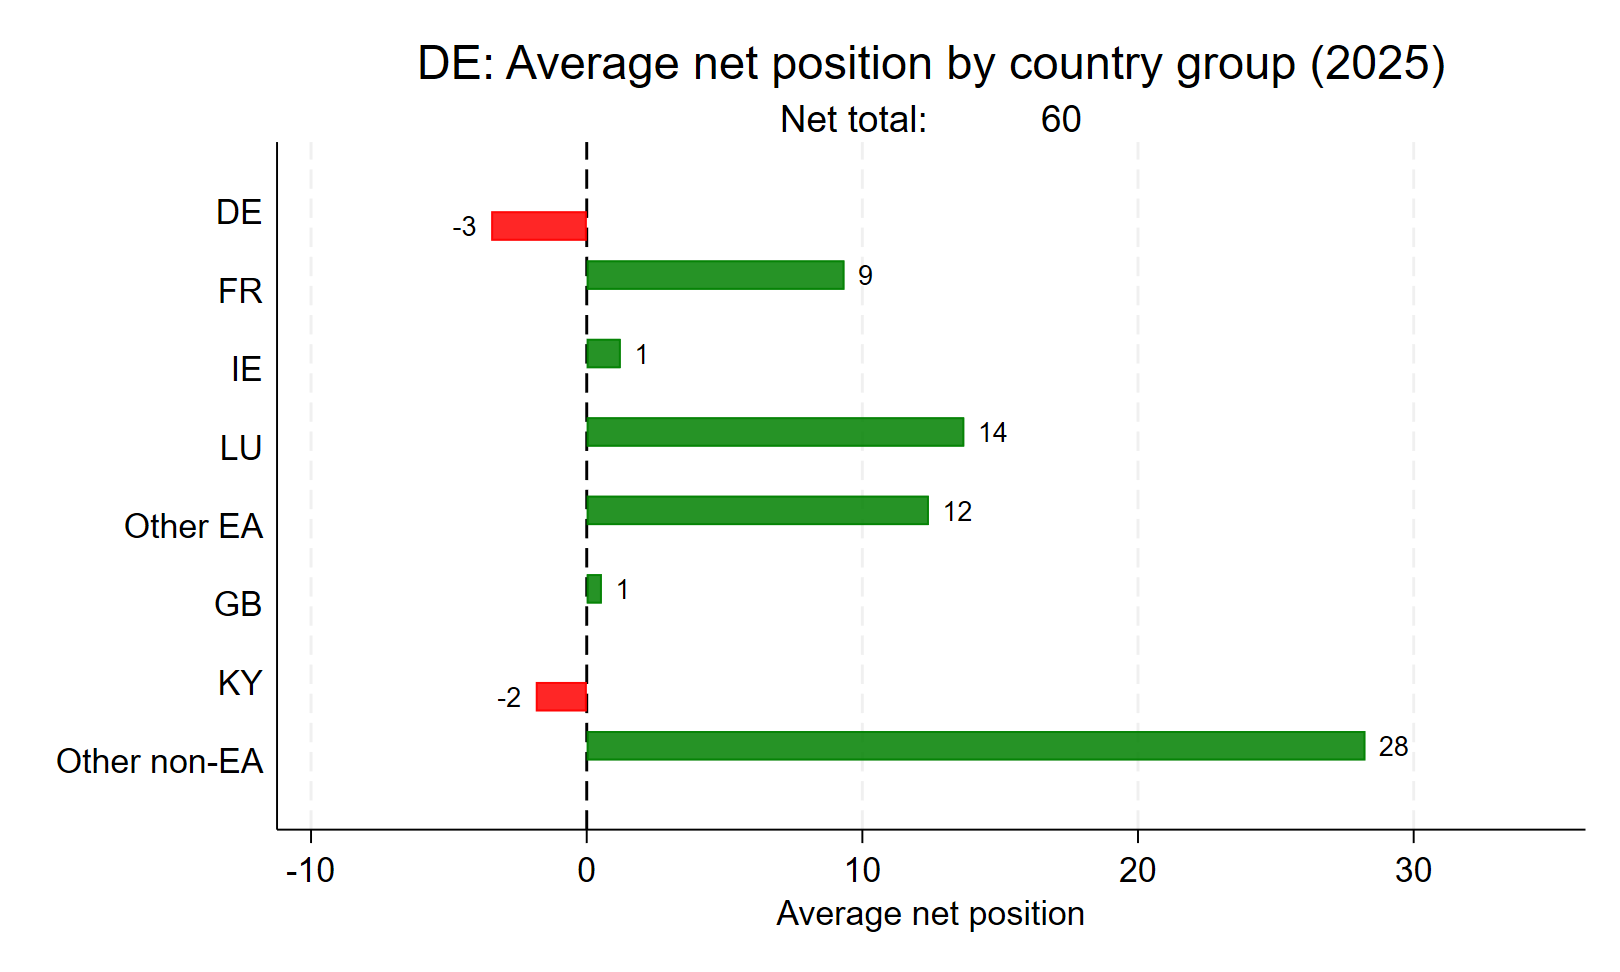
\includegraphics[width=1\linewidth]{Figures/DE_countries_2022.png}
\end{figure}

\begin{figure}\captionsetup{width=1\textwidth}
	\caption{\bf Fund locations - DE post 2025 }
	\caption*{\footnotesize
     This figure 
}
		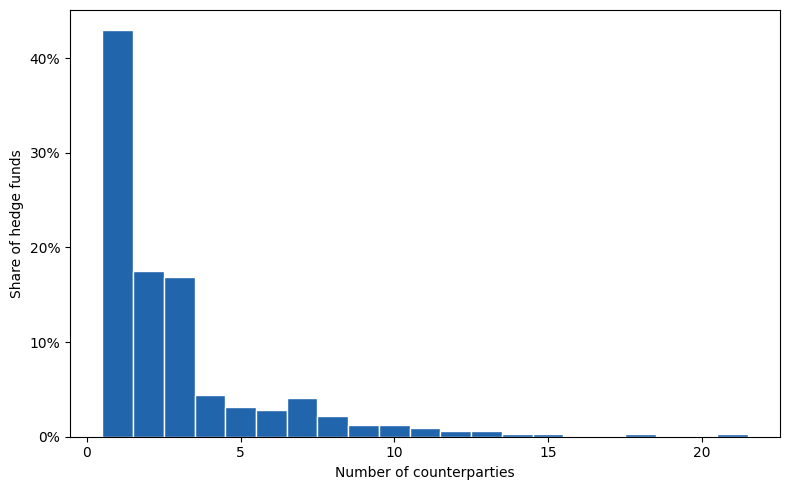
\includegraphics[width=1\linewidth]{Figures/DE_countries_2025.png}
\end{figure}


\begin{figure}\captionsetup{width=1\textwidth}
	\caption{\bf Fund locations - US pre 2023 }
	\caption*{\footnotesize
     This figure 
}
		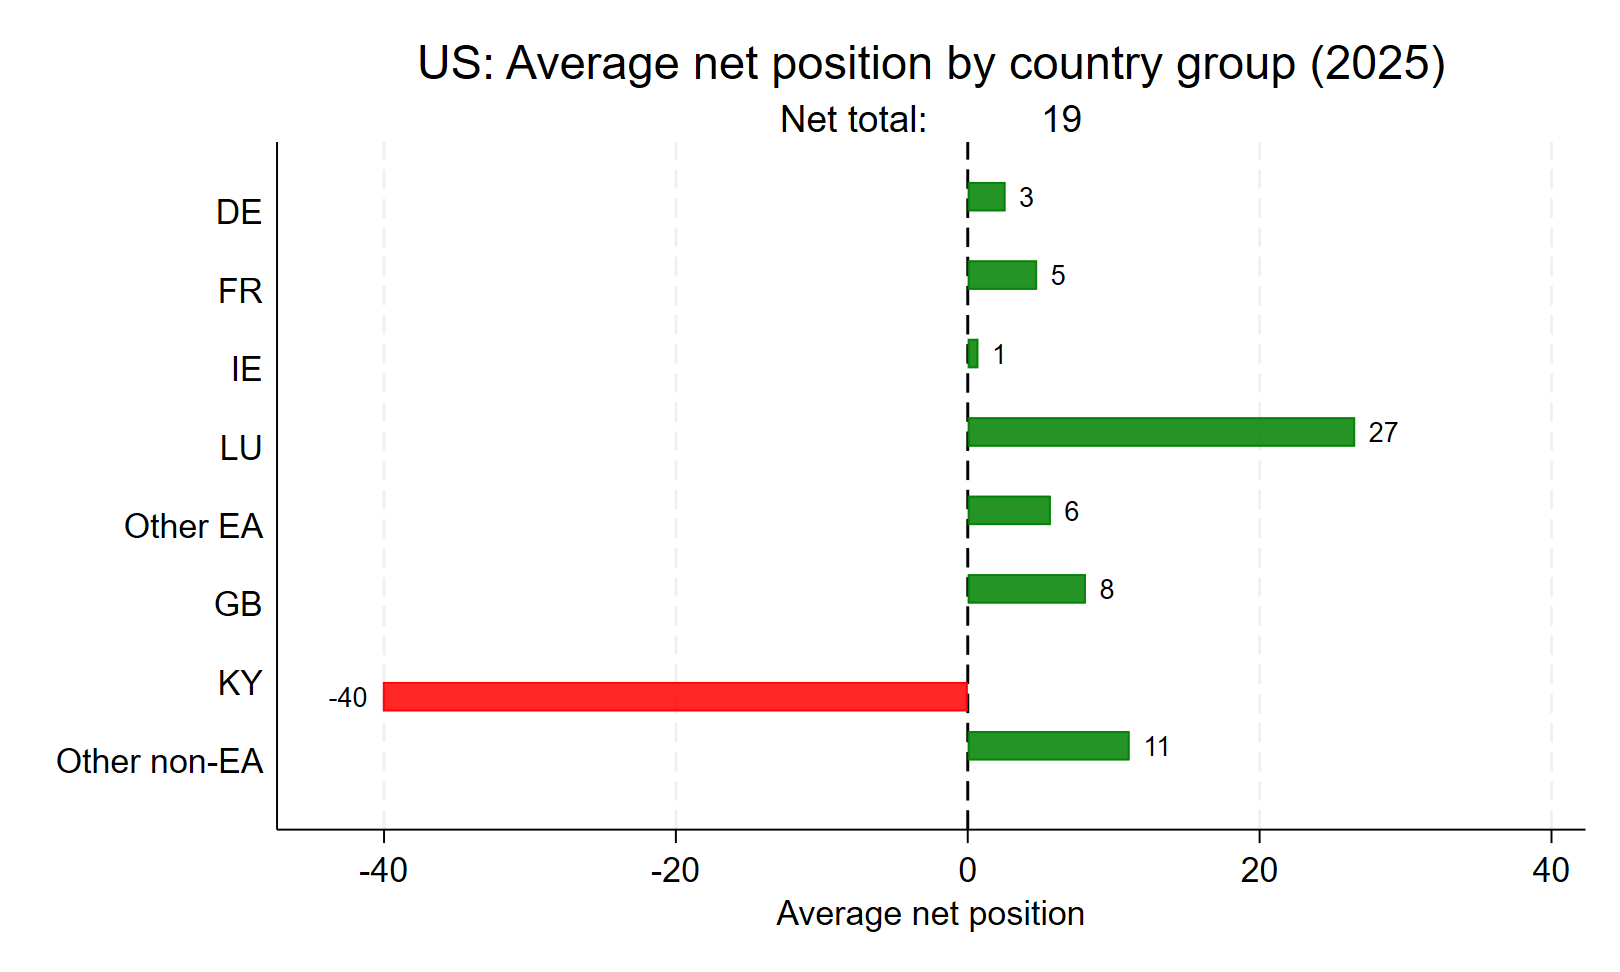
\includegraphics[width=1\linewidth]{Figures/US_countries_2022.png}
\end{figure}

\begin{figure}\captionsetup{width=1\textwidth}
	\caption{\bf Fund locations - US post 2025 }
	\caption*{\footnotesize
     This figure 
}
		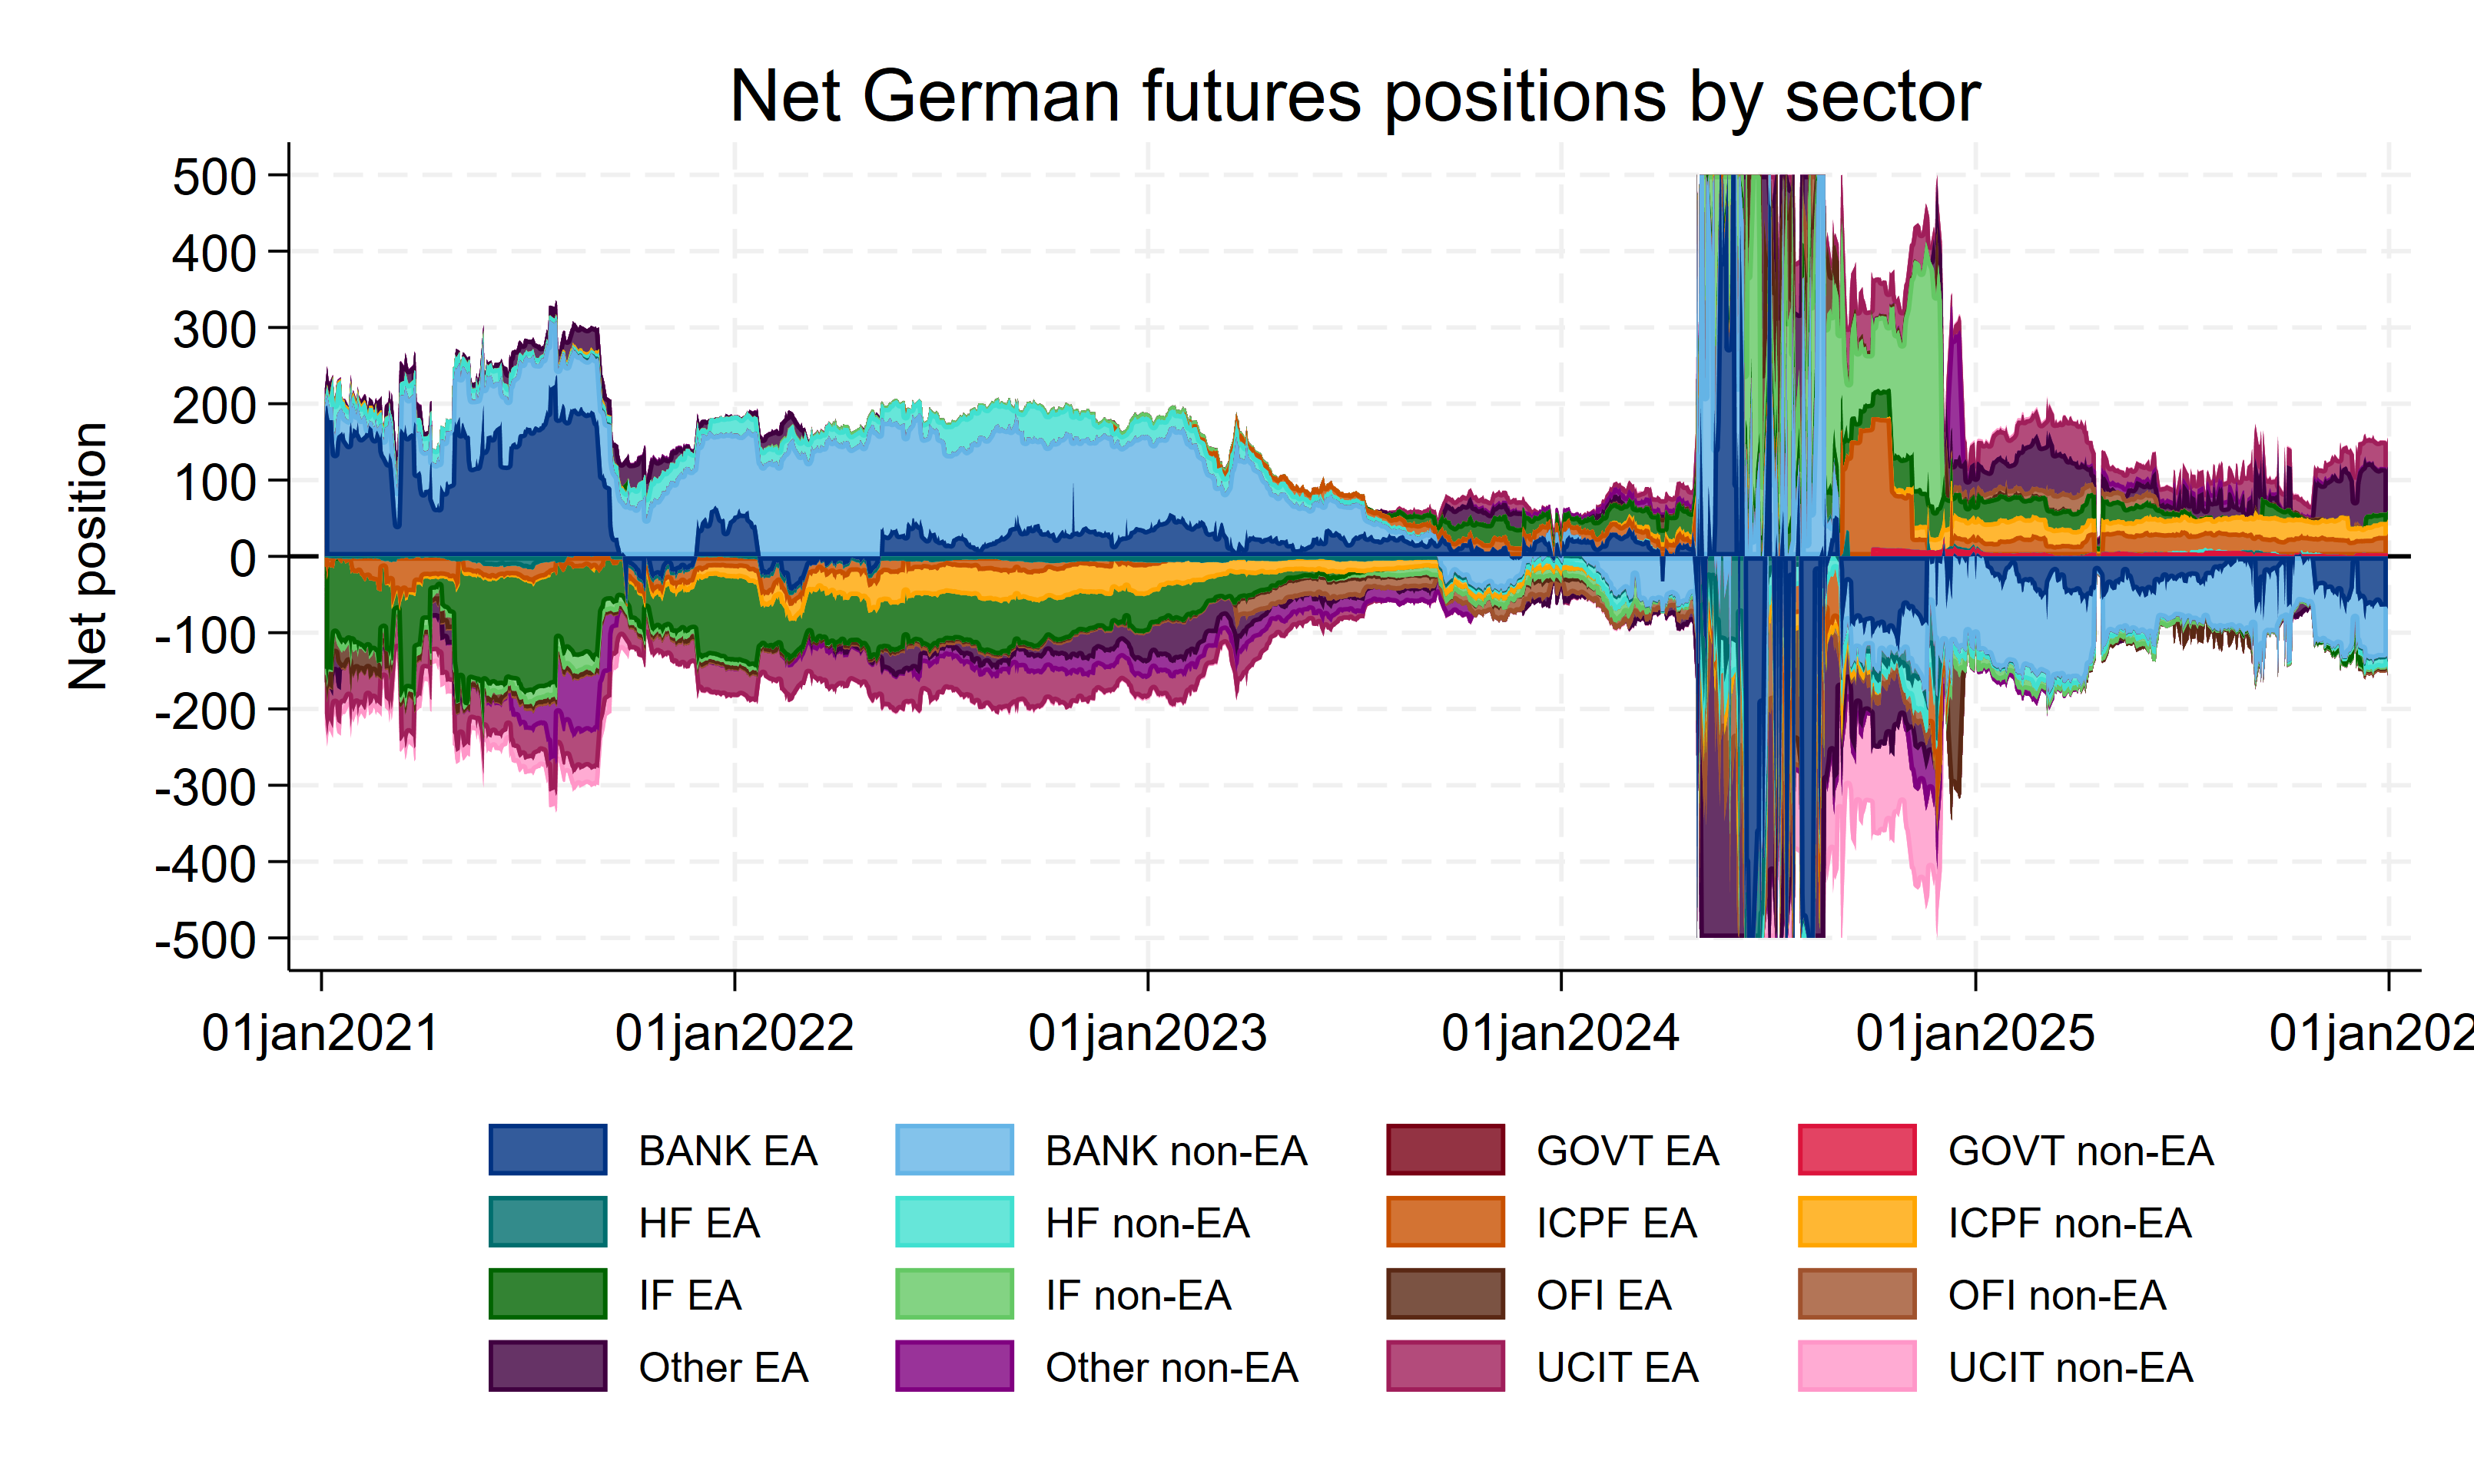
\includegraphics[width=1\linewidth]{Figures/US_countries_2025.png}
\end{figure}


\begin{figure}\captionsetup{width=1\textwidth}
	\caption{\bf Net positions - all euro area government bond futures}
	\caption*{\footnotesize
     This figure 
}
		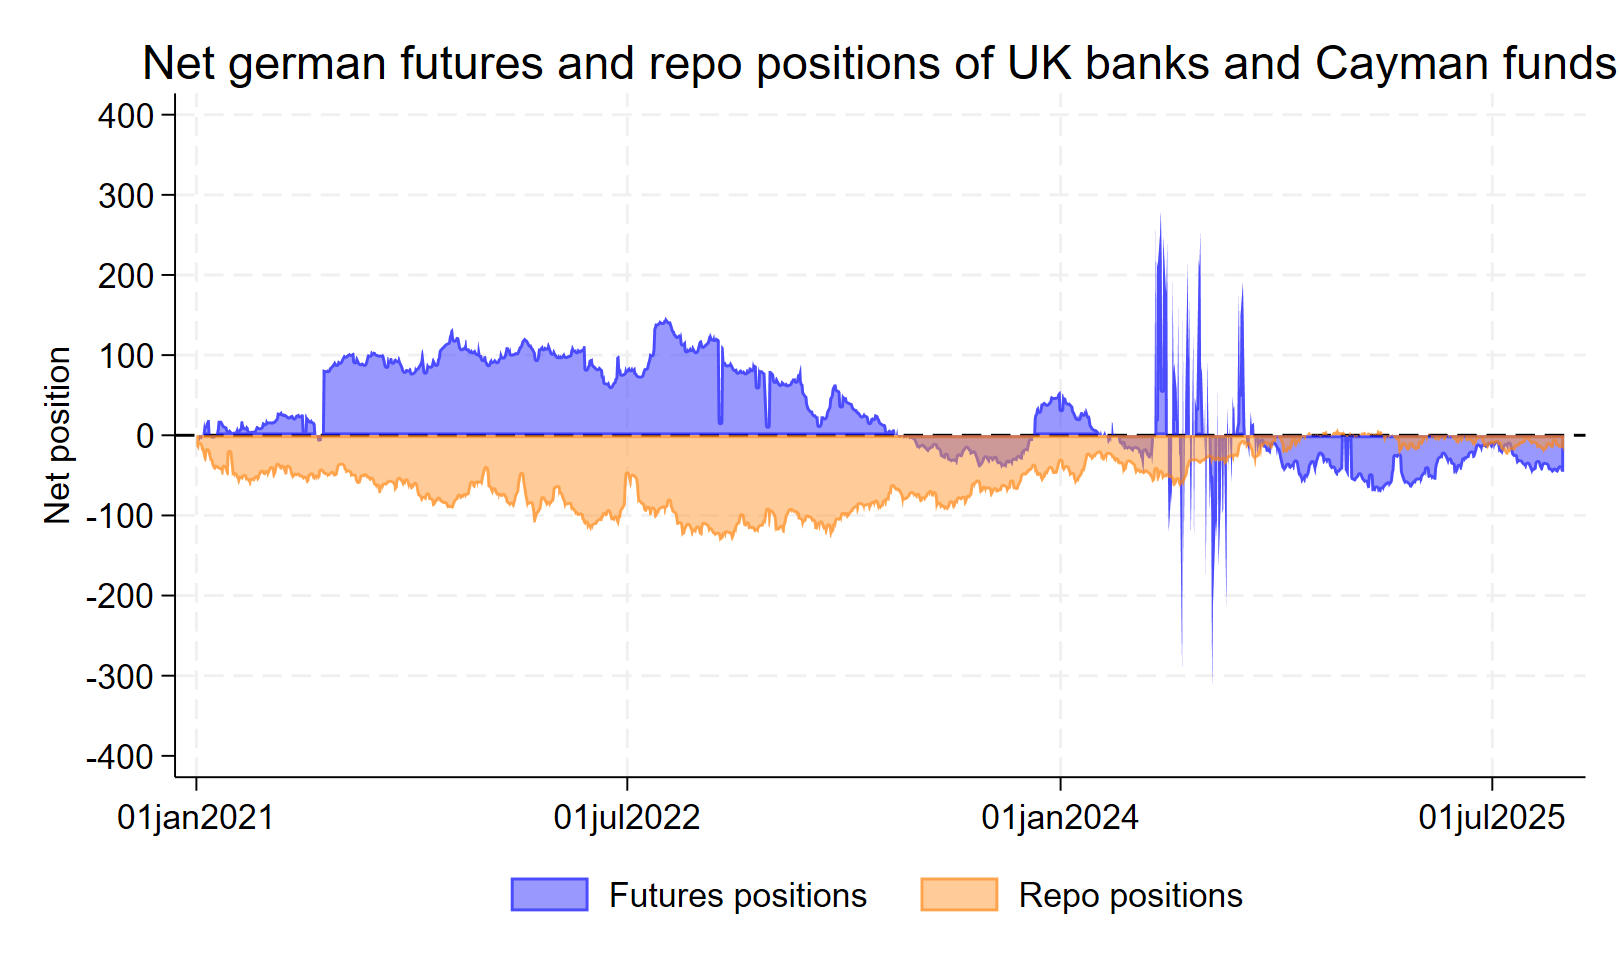
\includegraphics[width=1\linewidth]{Figures/net_repo_futures_all.png}
\end{figure}

\begin{figure}\captionsetup{width=1\textwidth}
	\caption{\bf Net positions - german government bond futures}
	\caption*{\footnotesize
     This figure 
}
		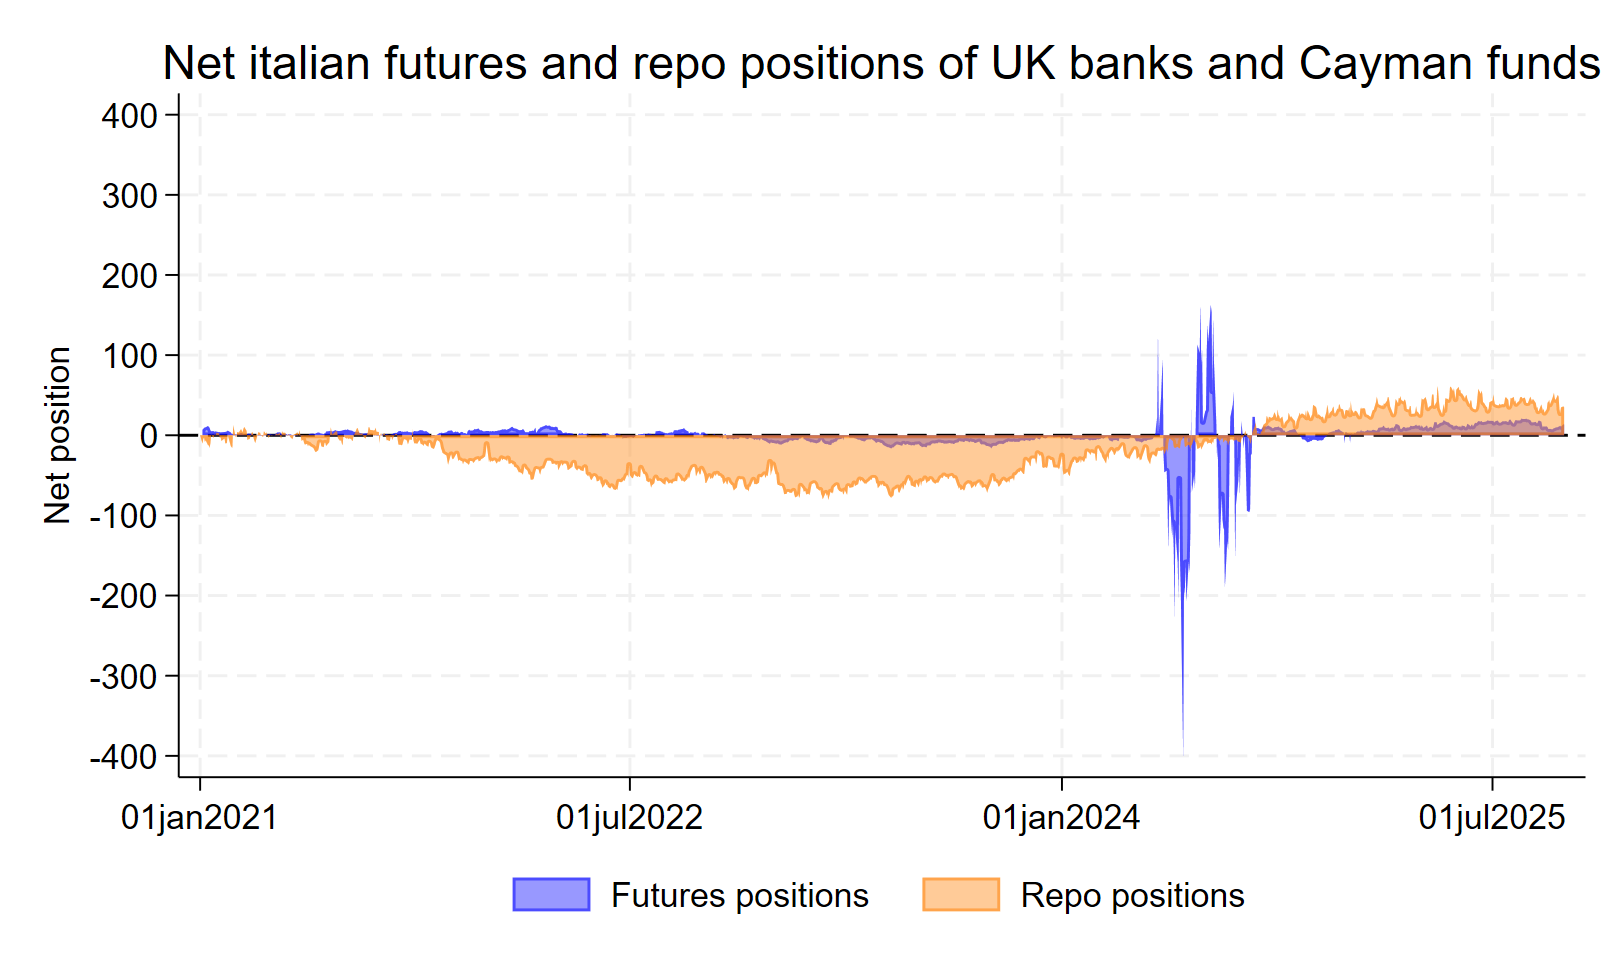
\includegraphics[width=1\linewidth]{Figures/net_repo_futures_DE.png}
\end{figure}


\begin{figure}\captionsetup{width=1\textwidth}
	\caption{\bf Net positions - italian government bond futures}
	\caption*{\footnotesize
     This figure 
}
		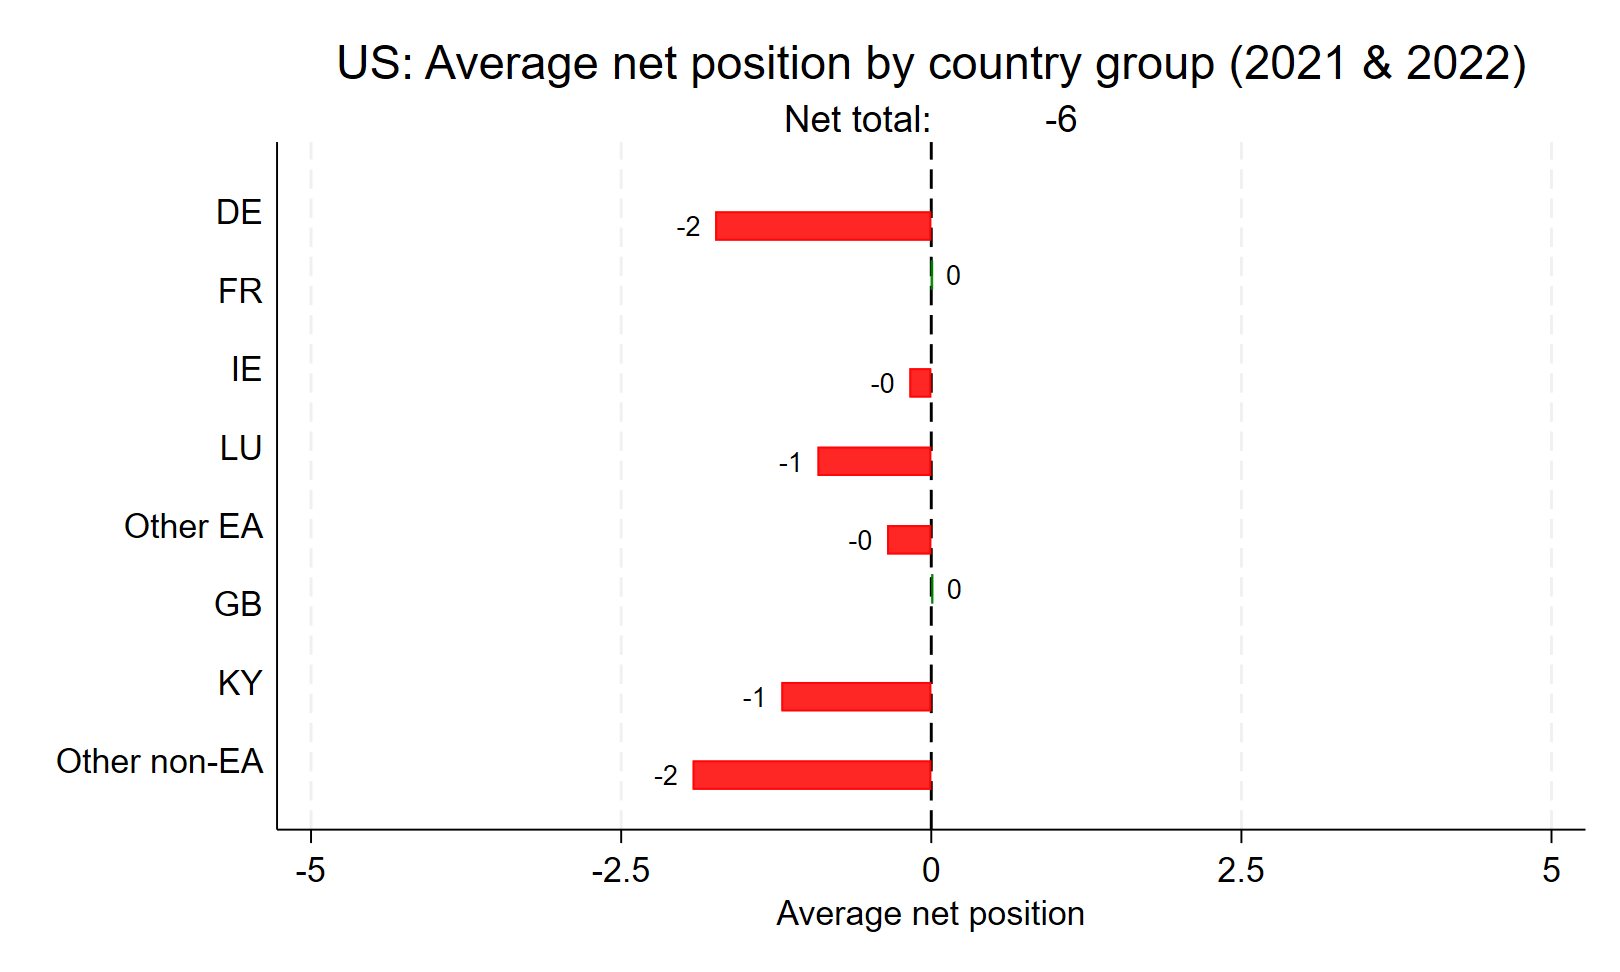
\includegraphics[width=1\linewidth]{Figures/net_repo_futures_IT.png}
\end{figure}


\begin{figure}\captionsetup{width=1\textwidth}
	\caption{\bf Net German futures positions by sector}
	\caption*{\footnotesize
     This figure 
}
		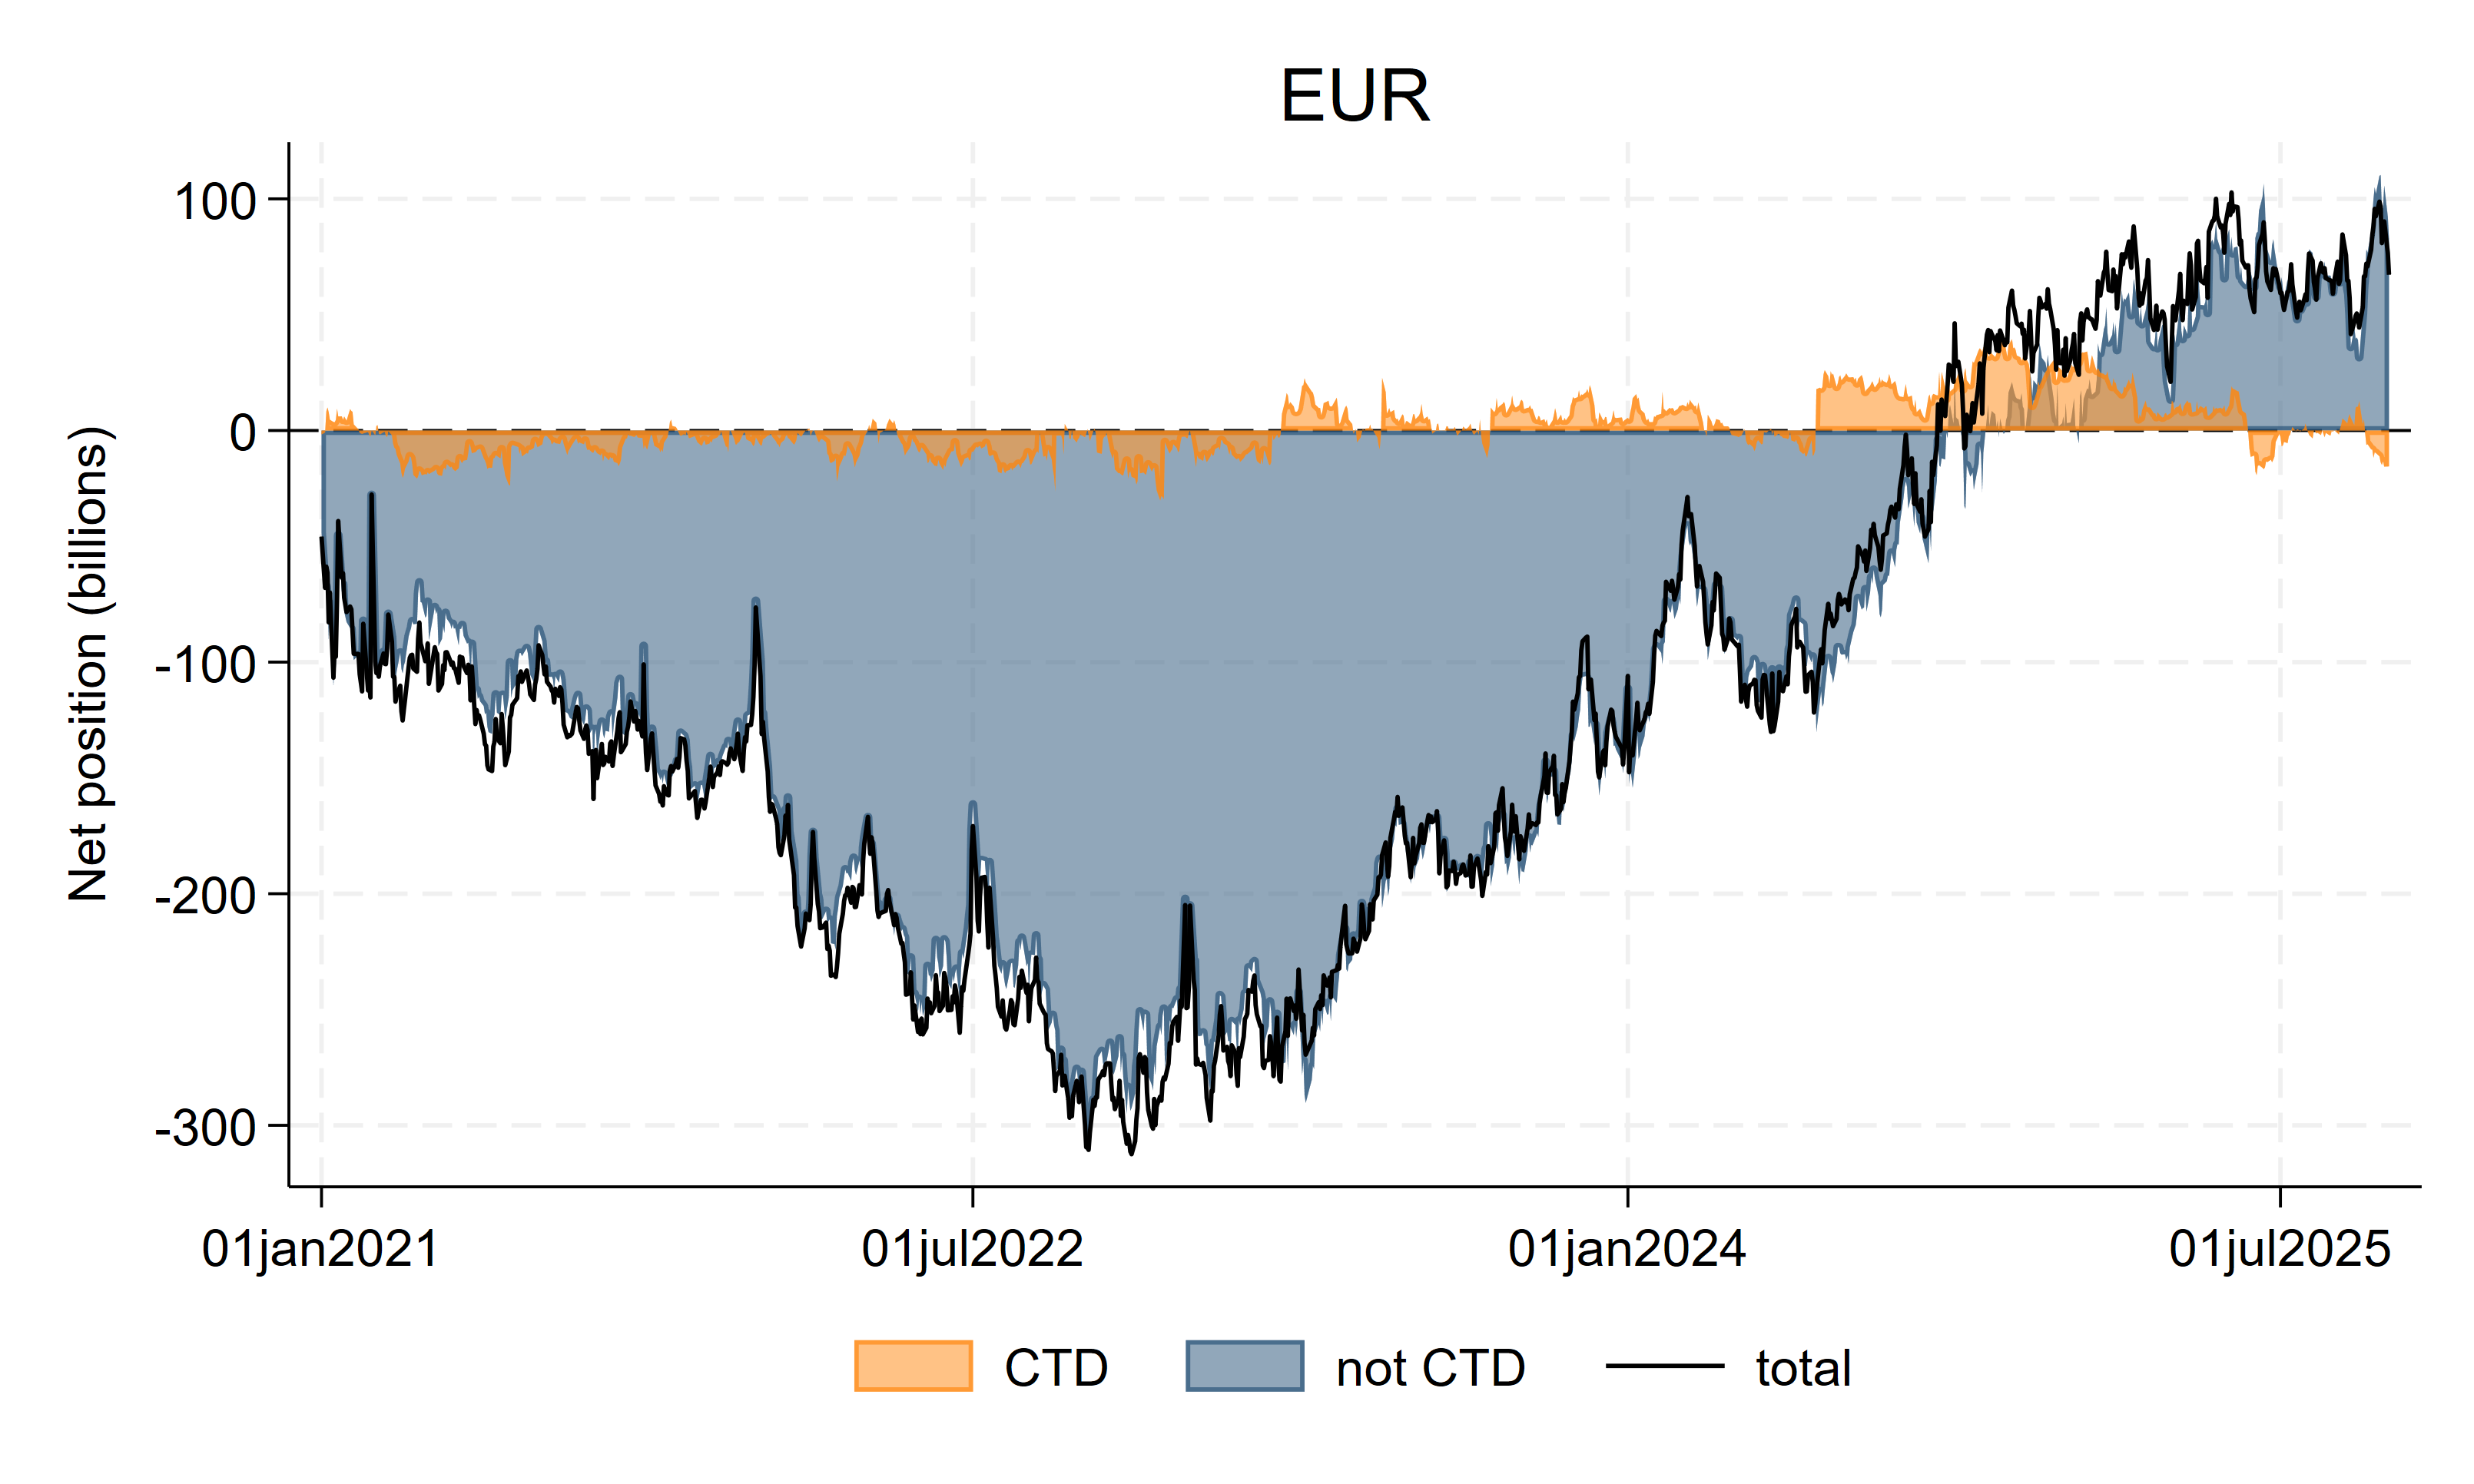
\includegraphics[width=1\linewidth]{Figures/sector_breakdown_german_futures.png}
\end{figure}



\begin{figure}\captionsetup{width=1\textwidth}
	\caption{\bf Net positions in OTR and other bonds}
	\caption*{\footnotesize
     This figure 
}
		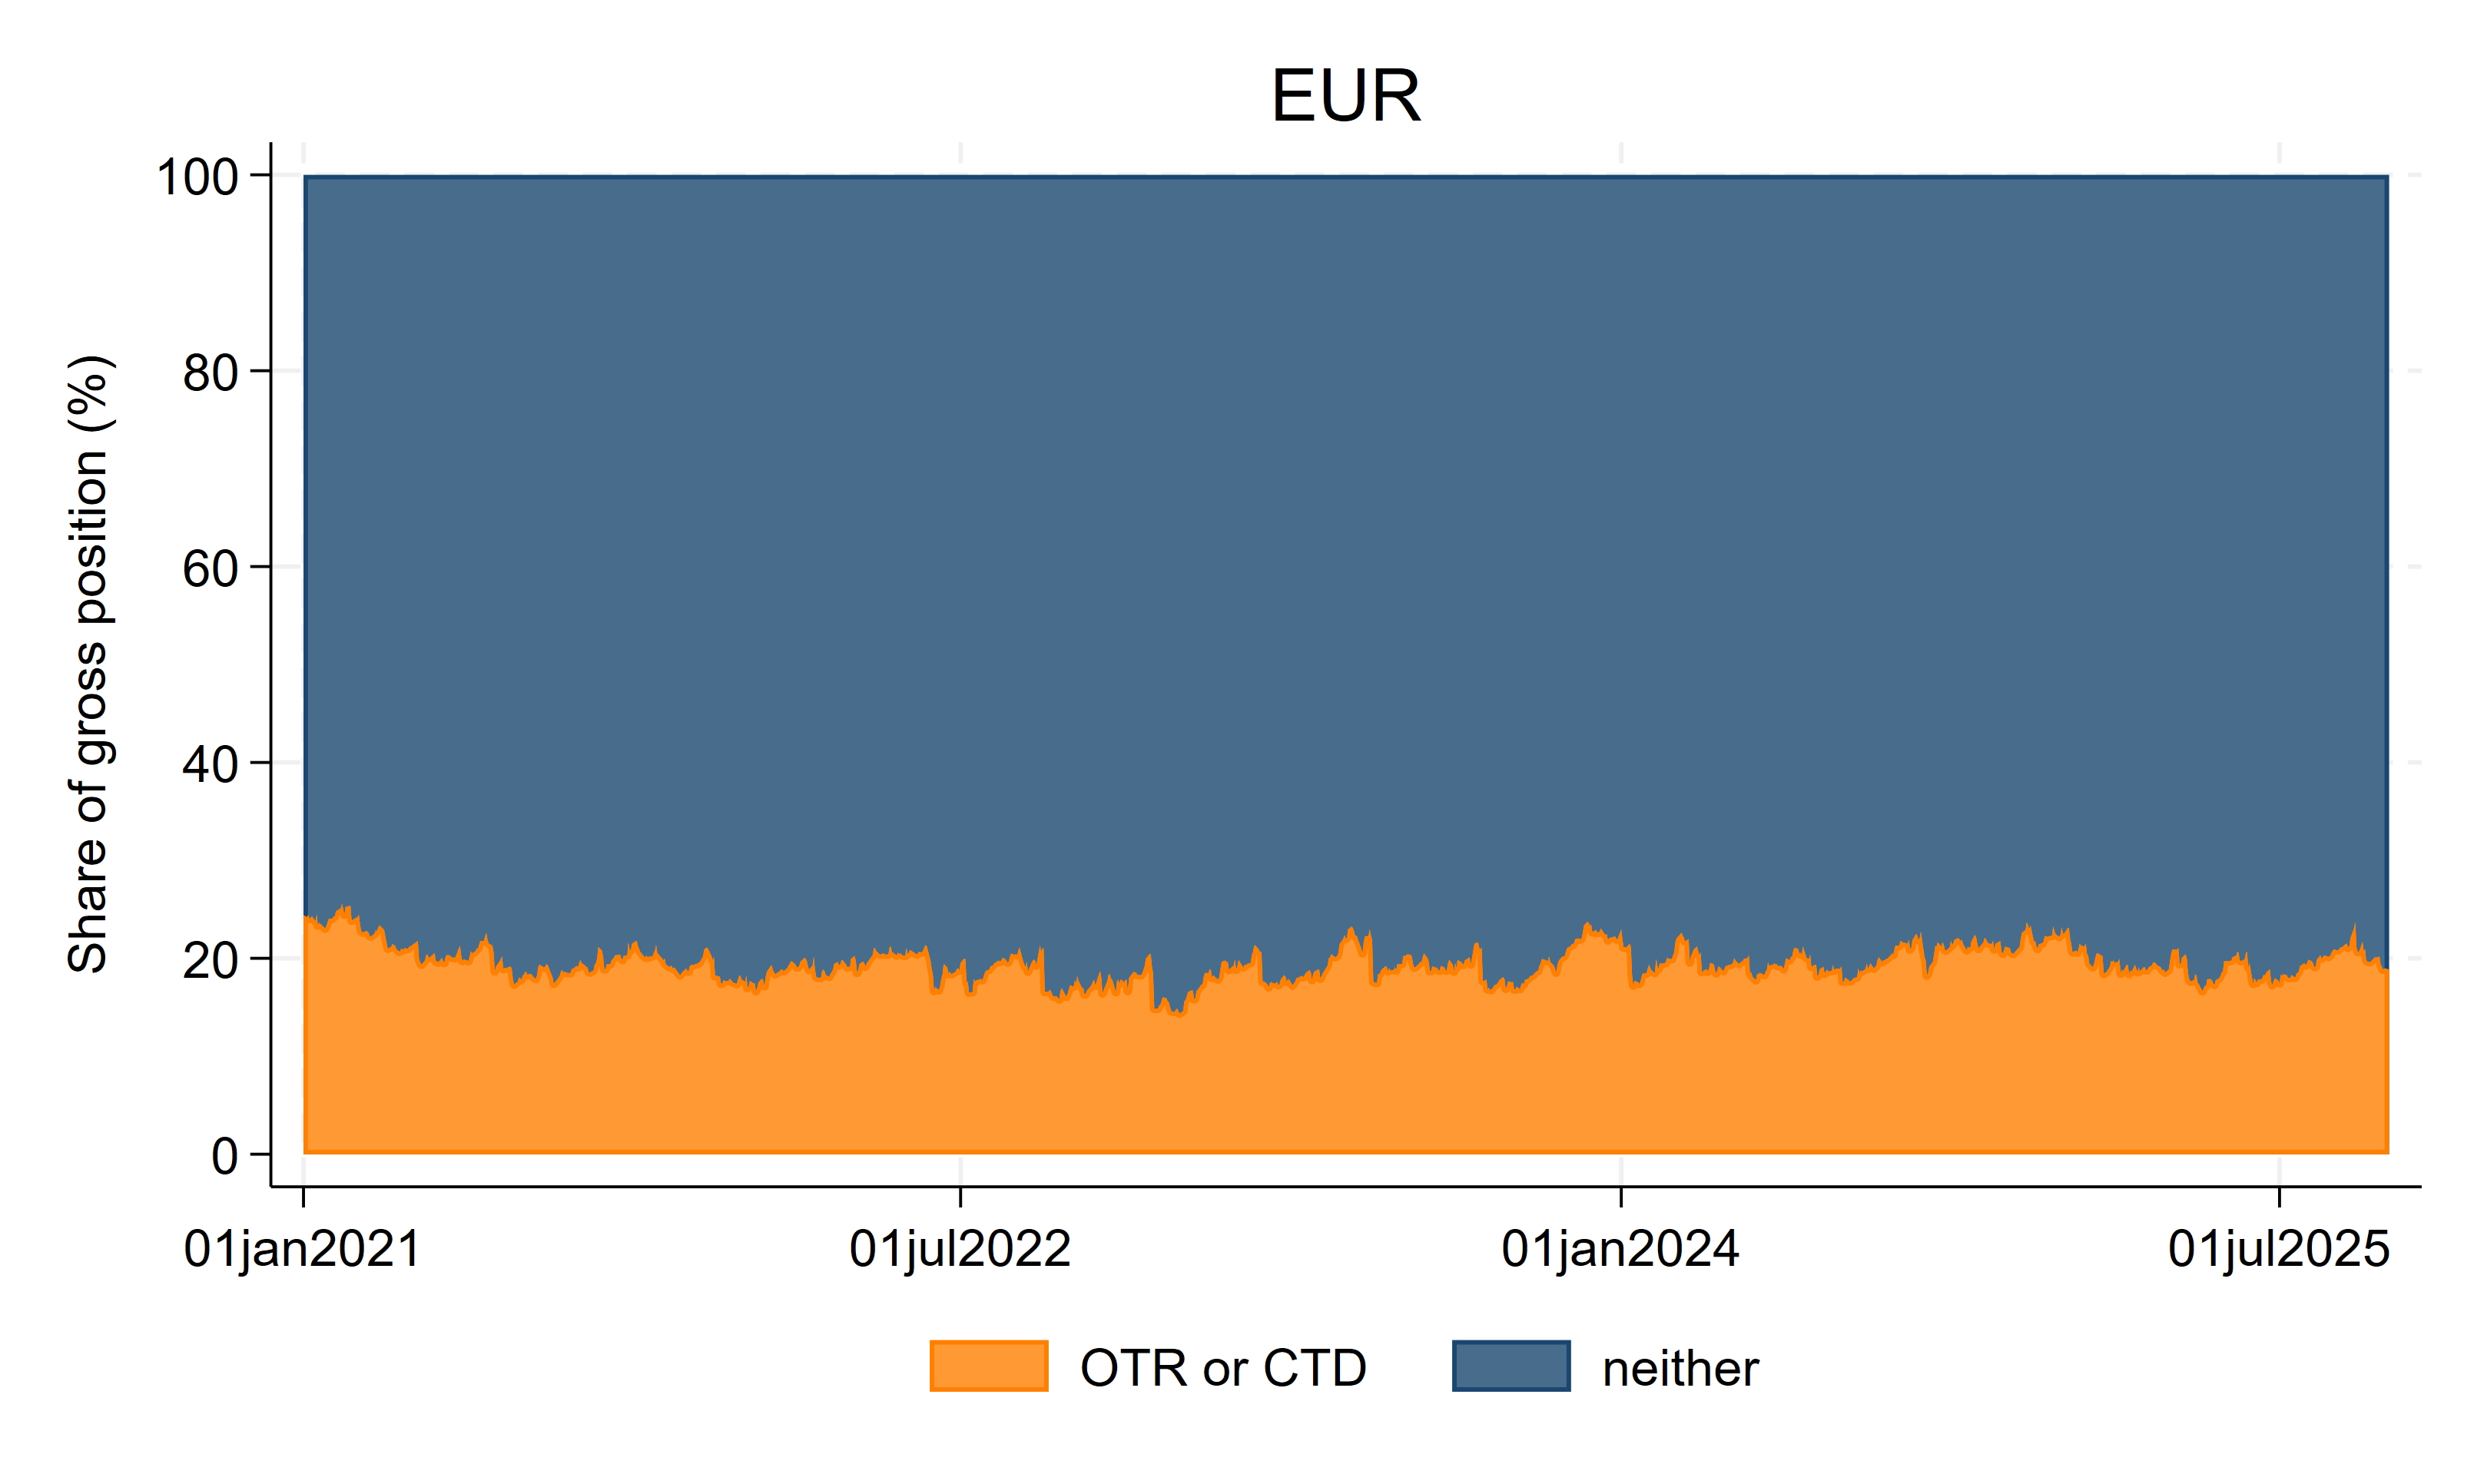
\includegraphics[width=1\linewidth]{Figures/EUR_otr.png}
\end{figure}

\begin{figure}\captionsetup{width=1\textwidth}
	\caption{\bf Net positions in OTR and other bonds}
	\caption*{\footnotesize
     This figure 
}
		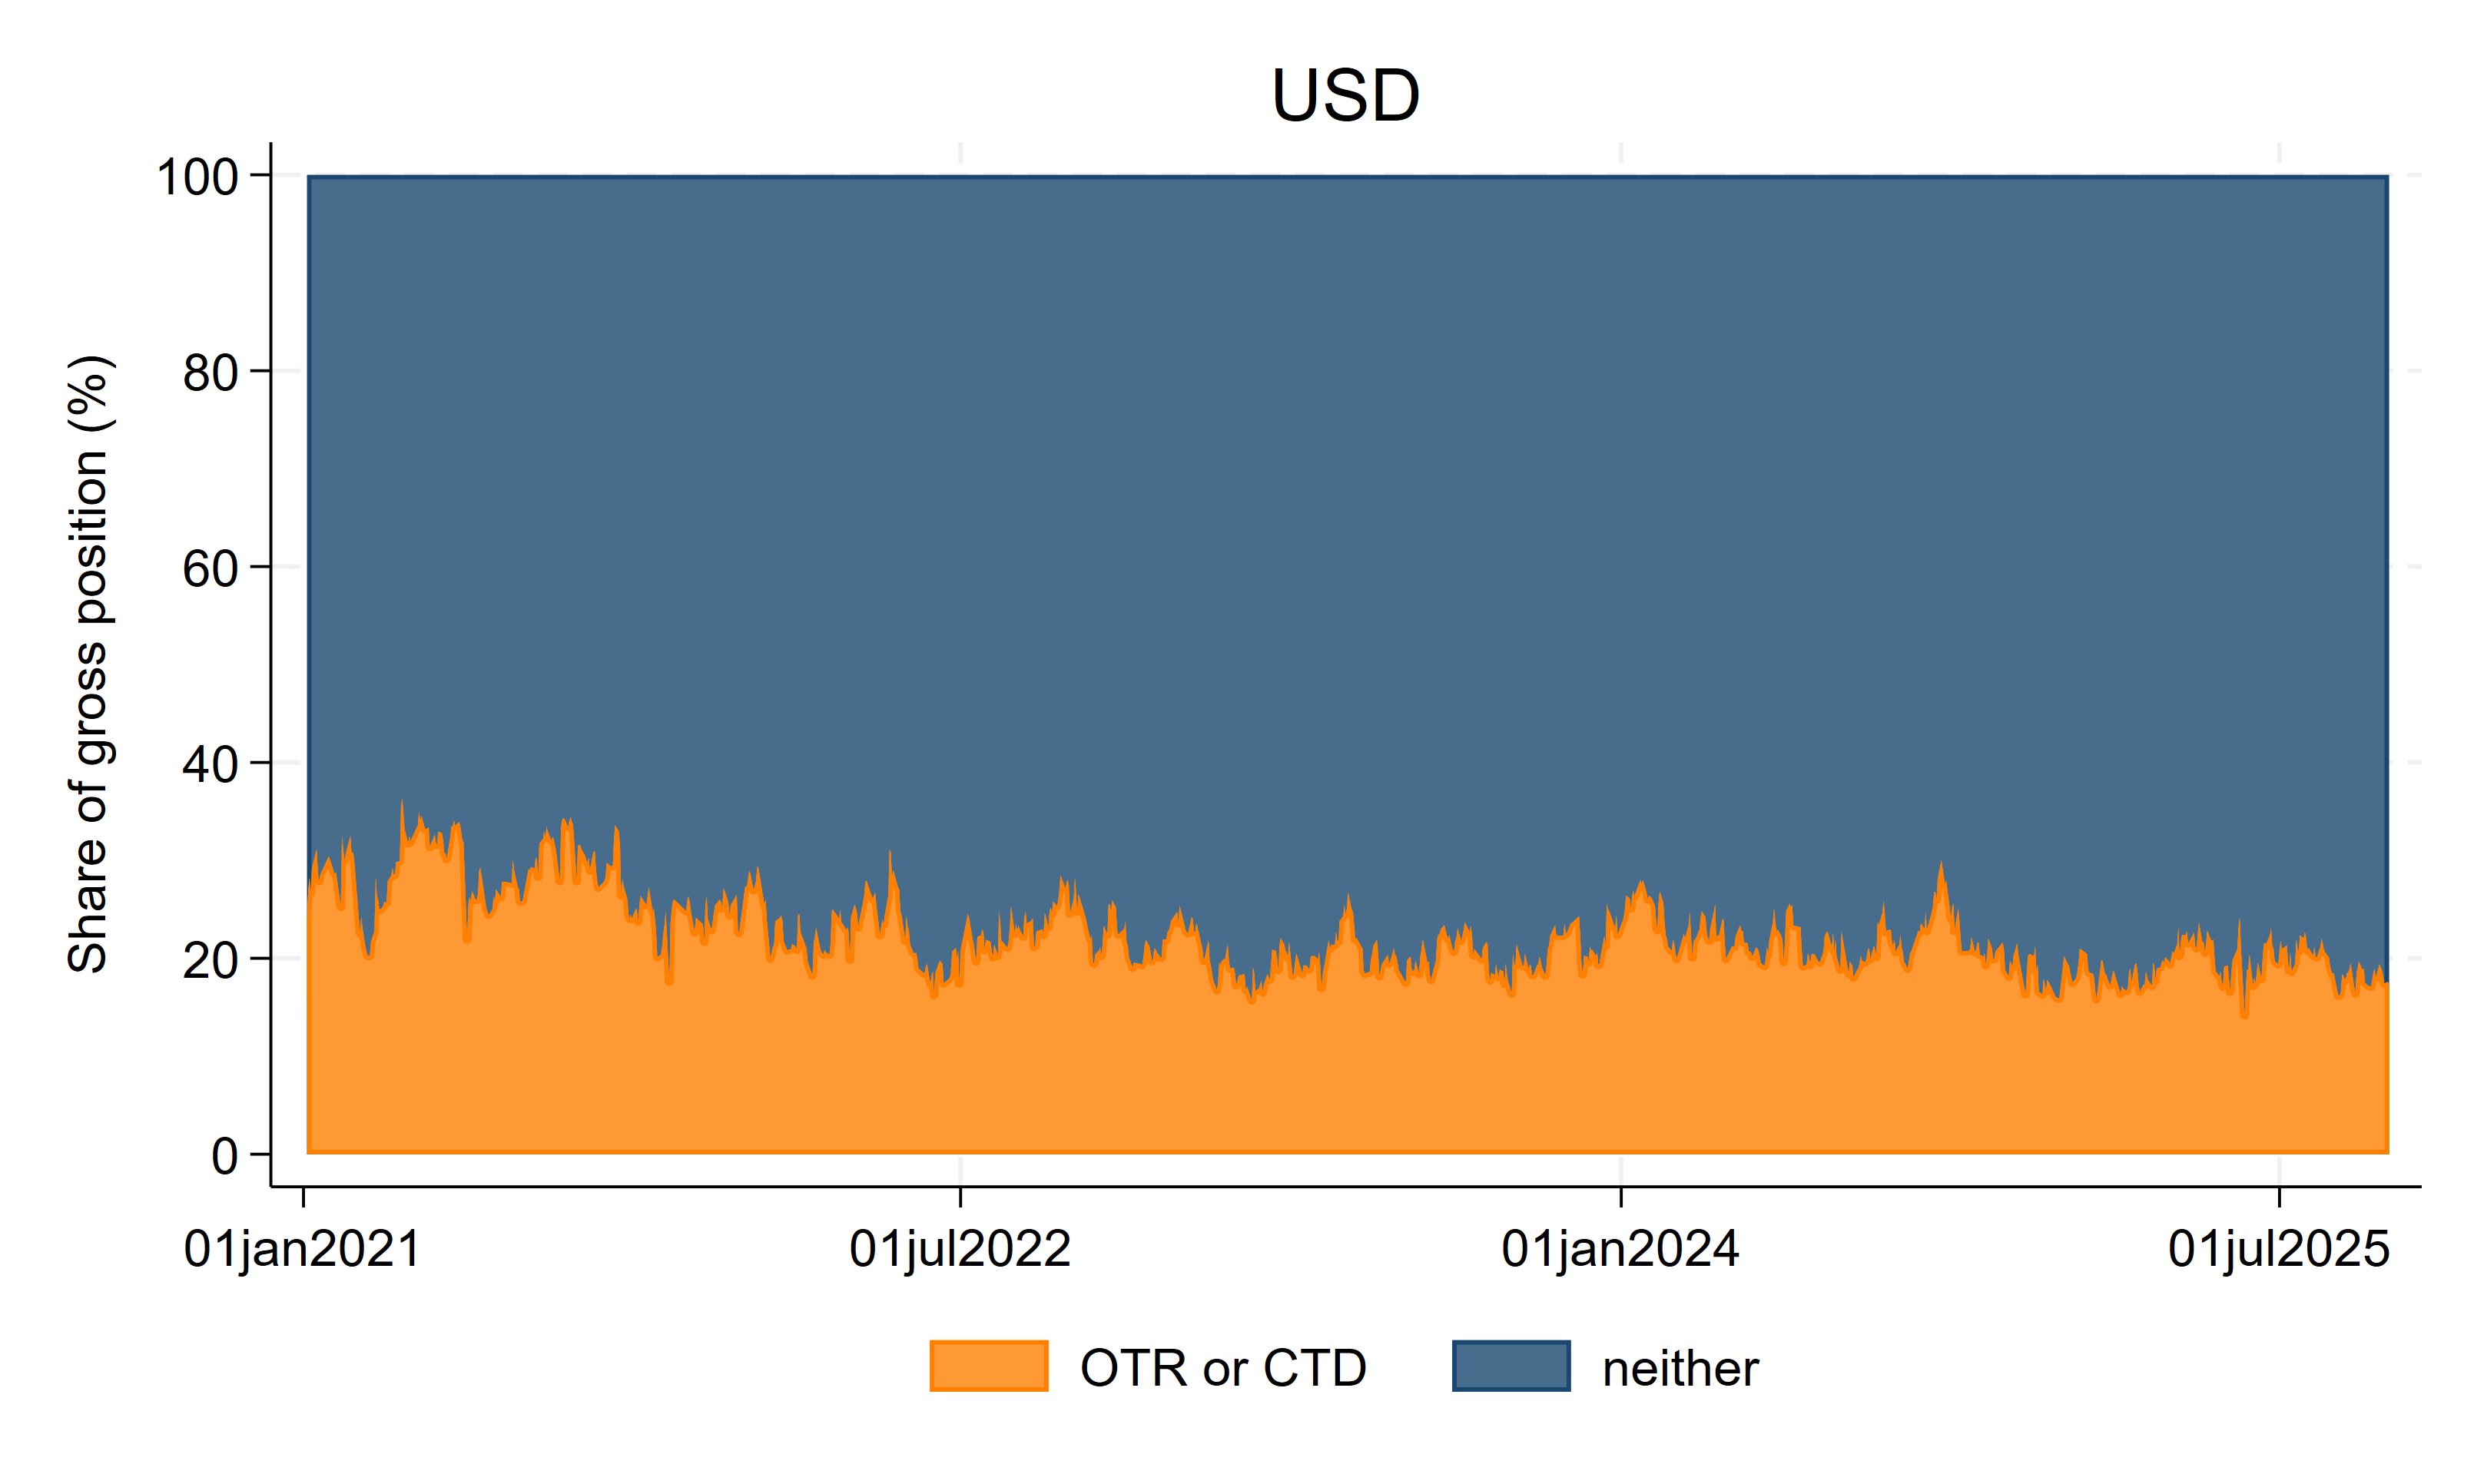
\includegraphics[width=1\linewidth]{Figures/USD_otr.png}
\end{figure}


\begin{figure}\captionsetup{width=1\textwidth}
	\caption{\bf Net positions in CTD and other bonds}
	\caption*{\footnotesize
     This figure 
}
		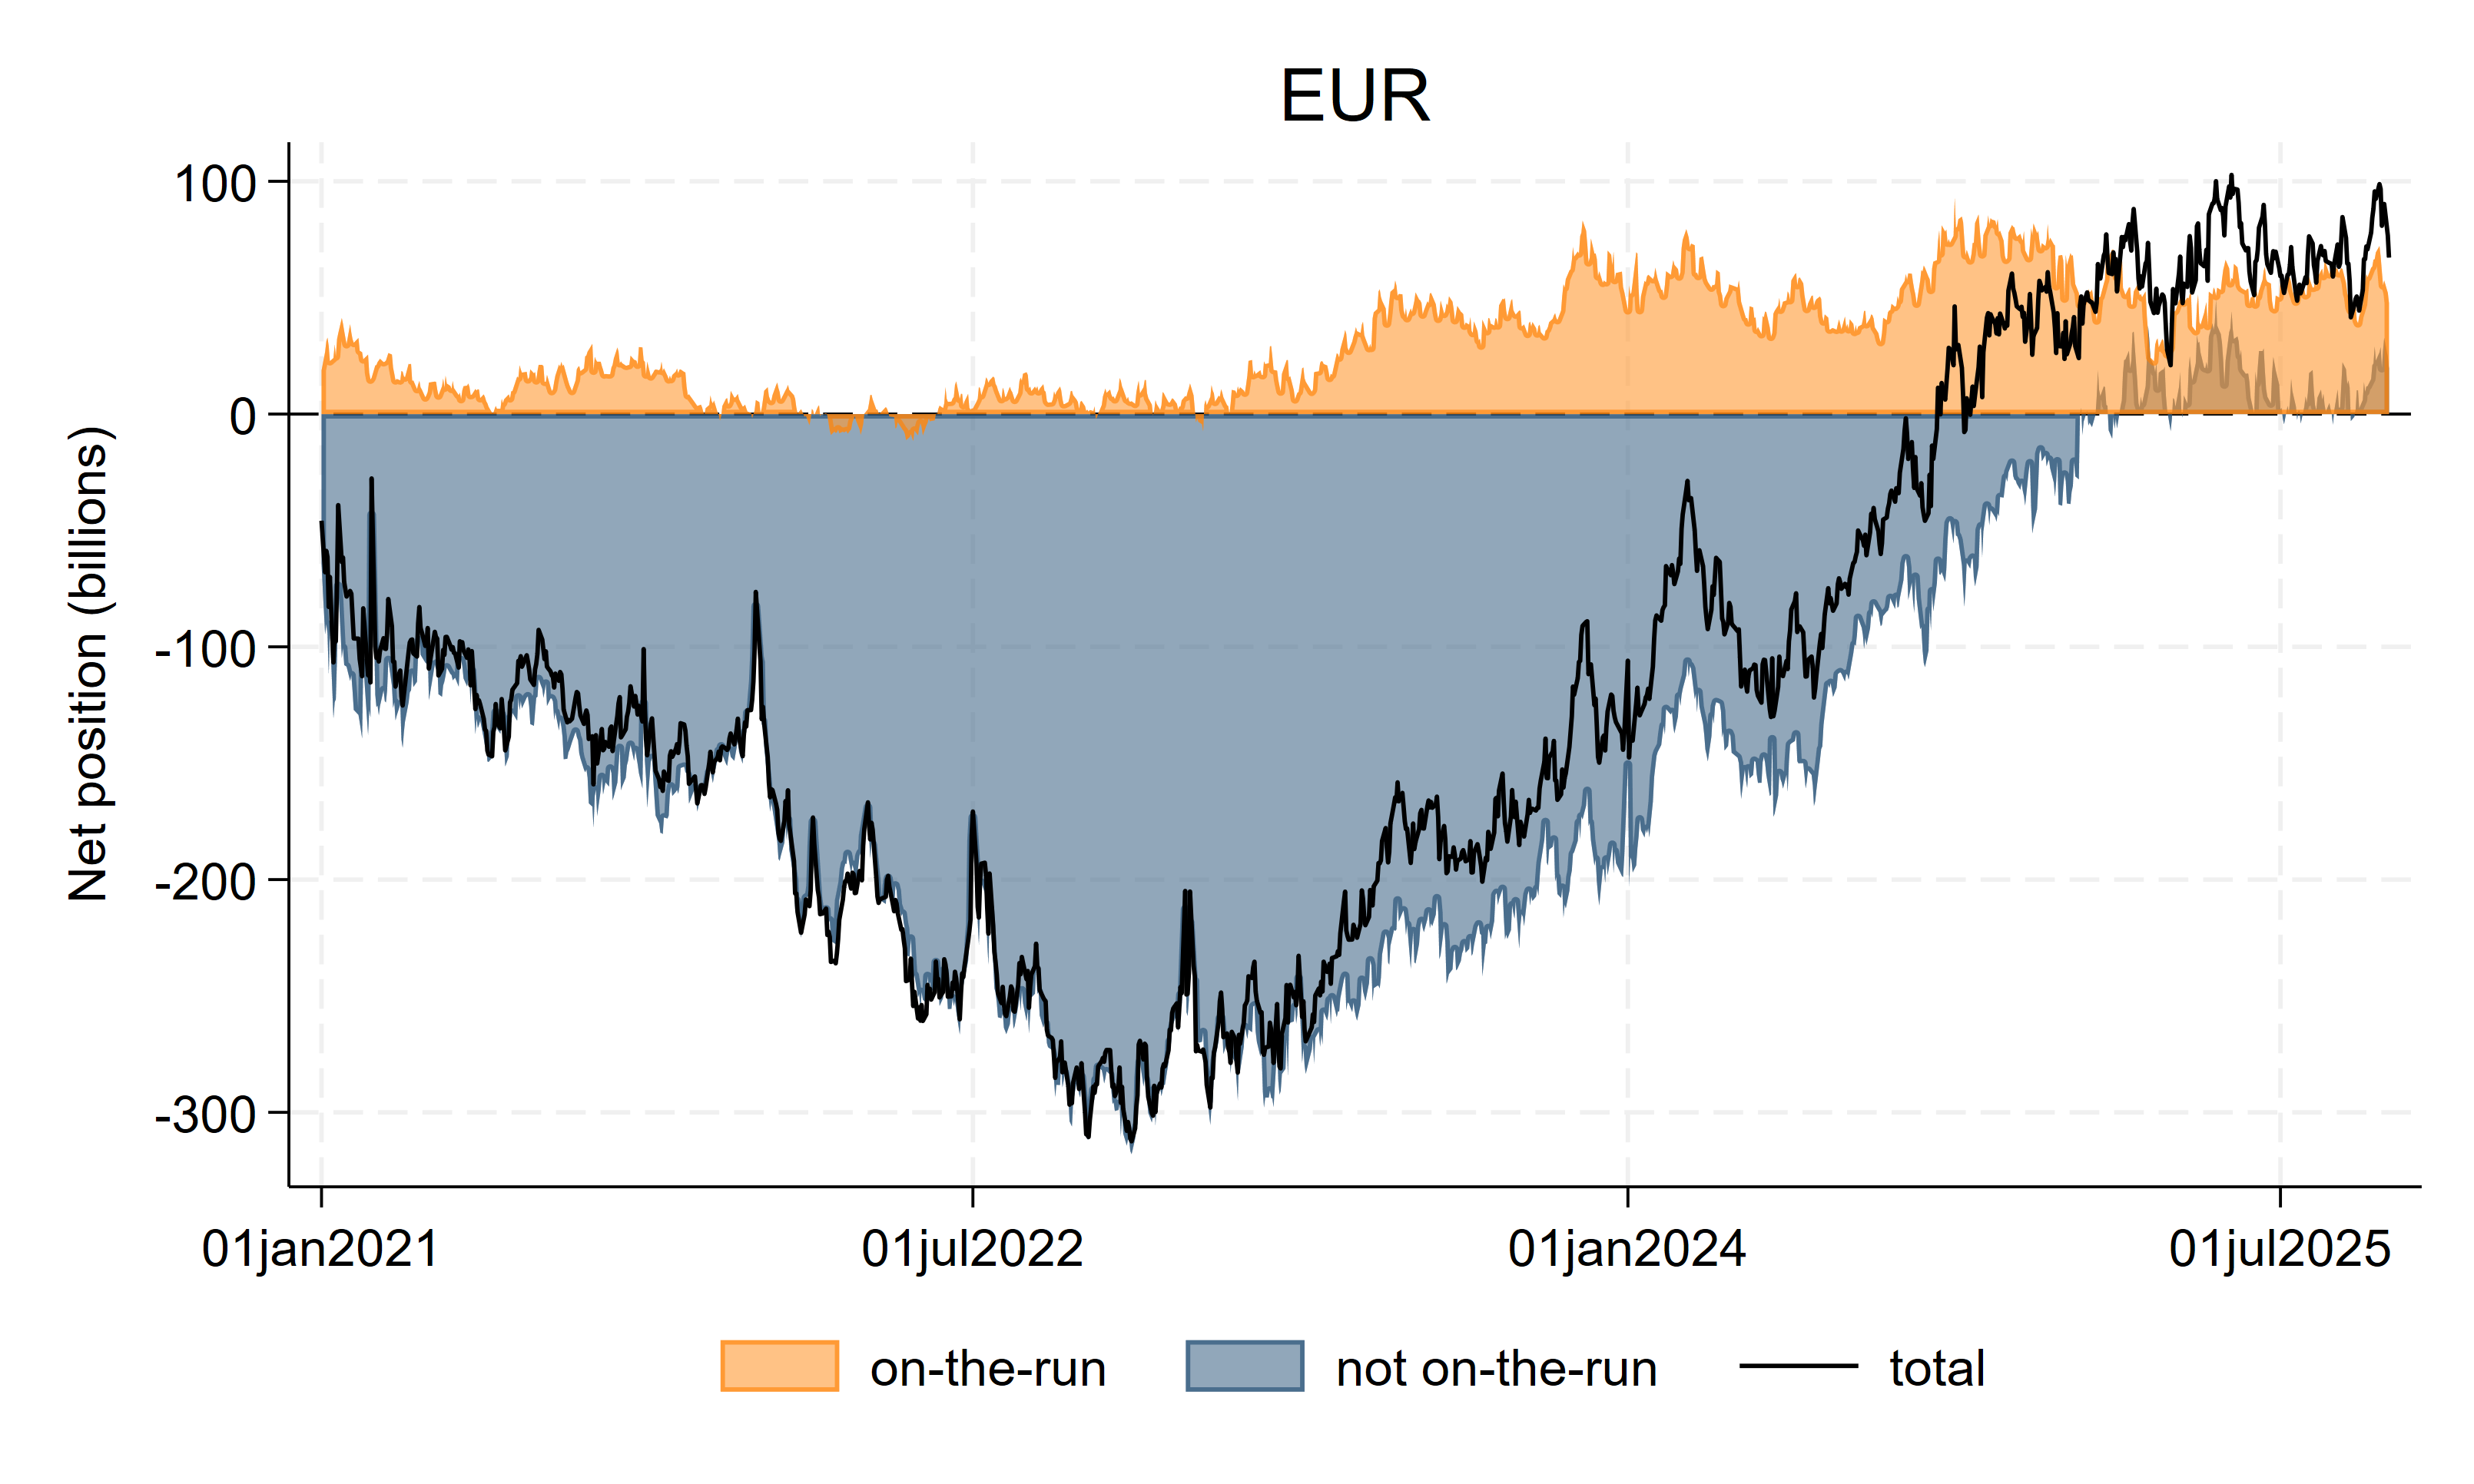
\includegraphics[width=1\linewidth]{Figures/EUR_ctd.png}
\end{figure}

\begin{figure}\captionsetup{width=1\textwidth}
	\caption{\bf Net positions in CTD and other bonds}
	\caption*{\footnotesize
     This figure 
}
		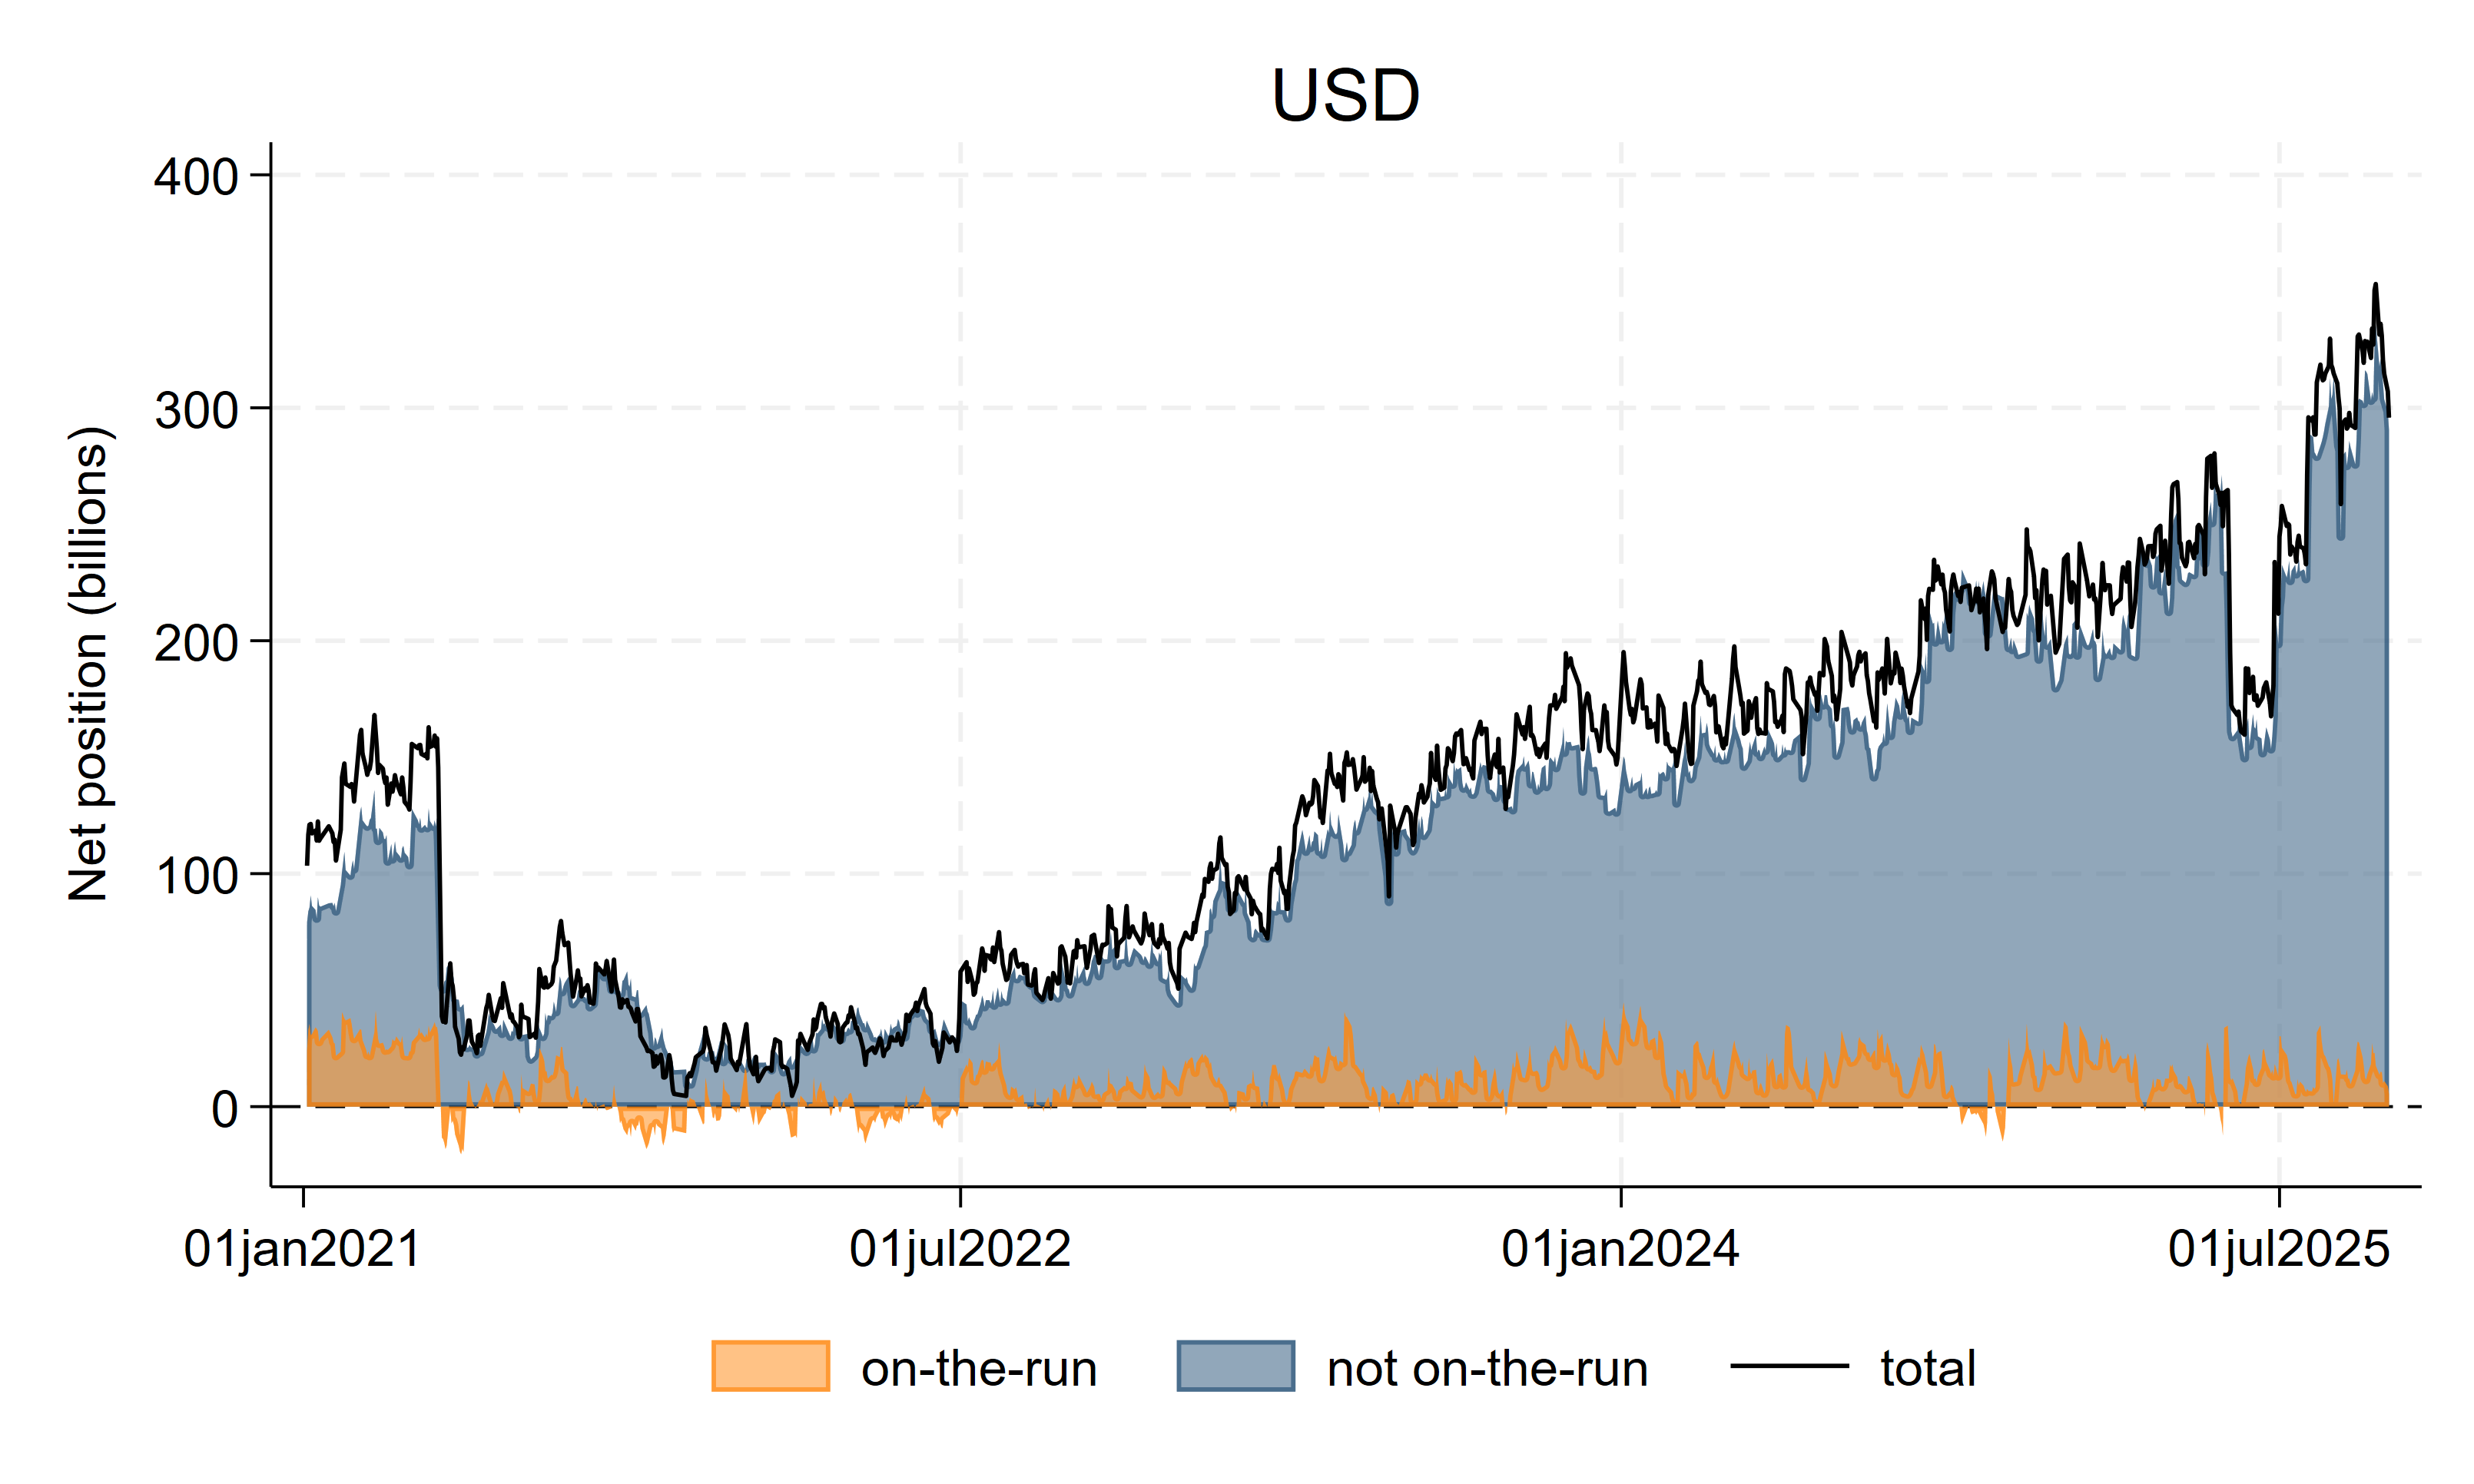
\includegraphics[width=1\linewidth]{Figures/USD_ctd.png}
\end{figure}


\begin{figure}\captionsetup{width=1\textwidth}
	\caption{\bf Share of gross positions in OTR/CTD bonds and others}
	\caption*{\footnotesize
     This figure 
}
		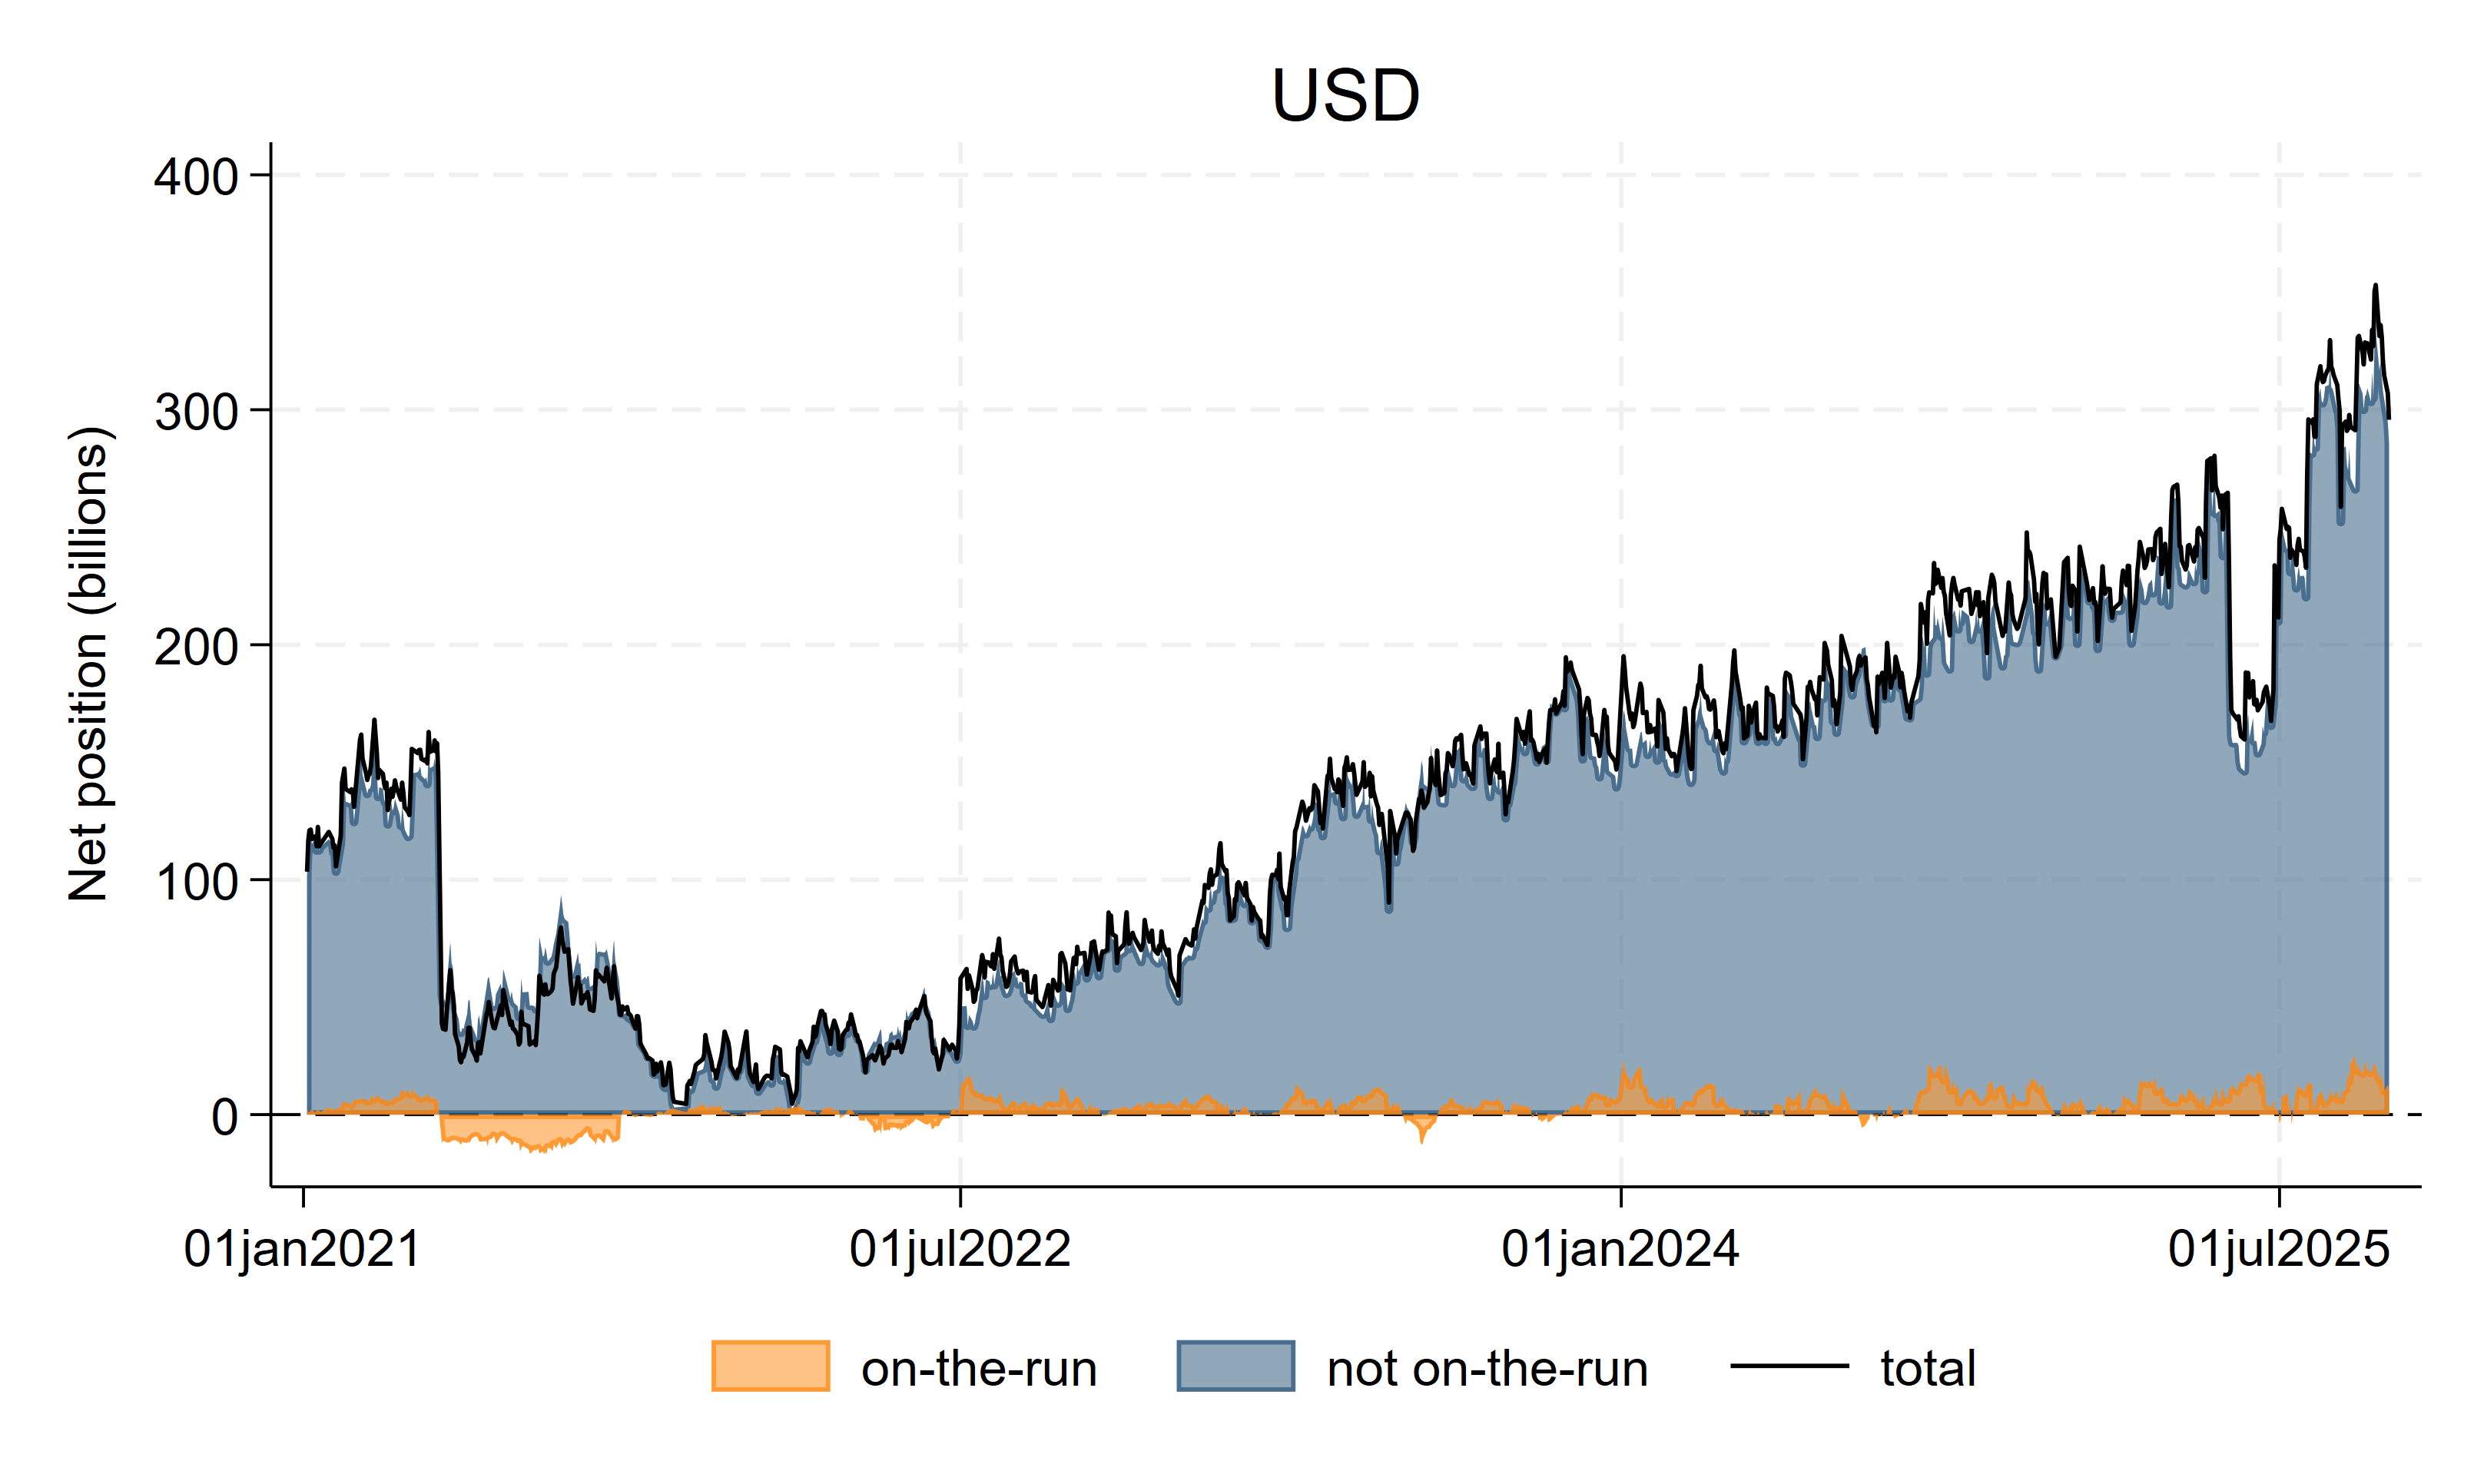
\includegraphics[width=1\linewidth]{Figures/EUR_otrctd_share.png}
\end{figure}

\begin{figure}\captionsetup{width=1\textwidth}
	\caption{\bf Share of gross positions in OTR/CTD bonds and others}
	\caption*{\footnotesize
     This figure 
}
		\includegraphics[width=1\linewidth]{Figures/USD_otrctd_share.png}
\end{figure}




\end{document}
